\chapter{Neural Network-Based Segmentation of Biomedical Images}
\label{chap:seg-background}

Image segmentation is the process of defining the borders of regions or objects on an image. For instance, delineating the liver from its surrounding tissue in a CT scan, separating each of a cell's organelles in a microscopic image, or determining the border between healthy and unhealthy tissue in a dermatoscopic image. This chapter introduces the different types of biomedical images as well as the process of segmenting them. We will first provide an overview of the world of biomedical images and its diverse modalities and imaging techniques. We will touch on the technical details of how these images are stored and used in segmentation algorithms. Then, we will more formally describe the process of image segmentation from traditional segmentation methods to the most current deep learning methods.

Biomedical imaging covers a wide range of techniques used in both biology and medicine \cite{Wallyn2019}. This includes complex modalities like CT scans and simpler ones like photographs of a patient's skin or plants. Because of this variety, a method designed for one modality might not work for another without changes. So, understanding each modality's specifics is crucial when considering segmentation methods. The next section will provide an overview of different biomedical imaging modalities, focusing on those most relevant to this thesis.

\section{Common Types of Biomedical Images}

Broadly, we may classify biomedical images into ones that have three and two spatial dimensions. Images with three spatial dimensions include modalities such as CT and MRI. Examples of image modalities with two spatial dimensions, among others, include X-ray imaging, most microscopic images, and dermatoscopic images. Images from both of these categories can also include additional dimensions such as time. It is worth noting that biomedical images do not always fit neatly into distinct categories. While our classification provides a general overview, there are emerging techniques that merge different modalities \cite{strangmanQuantitativeComparisonSimultaneous2002}, blurring the classification boundaries presented here.

\subsection{3D Modalities}

It is hard to overstate the importance of 3D modalities such as CT and MRI in contemporary medical practice, scientific advancements, and patient outcomes \cite{Wallyn2019}. These techniques offer medical professionals a window into the patient's body, allowing much safer and more reliable diagnosis, treatment, and surgical planning. 

The foundational principle behind these modalities revolves around emitting a signal capable of penetrating tissues. This signal interacts variably with different tissue types. After transmission through the body, the residual signal is detected and used to create an image. By repeating this process across various planes of the body and leveraging computational algorithms, a 3D volume of the patient's anatomy is constructed. From there, these modalities are often stored as voxel-based 3D files, where a voxel is the smallest 3D unit equivalent to a pixel in 2D images. They are usually stored alongside patient data such as age, sex, imaging parameters, and other relevant information.

In the subsequent sections, we will delve deeper into the specifics of the two predominant 3D biomedical imaging modalities: CT and MRI.

\subsubsection{Computed Tomography (CT)}

Computed tomography is an X-ray-based imaging technique where different planes of the subject are captured and then reconstructed into a 3D image using a process called tomography \cite{goldmanPrinciplesCTCT2007}. CT, as opposed to MRI, uses ionizing radiation that can be harmful in large doses. As such, the benefit of each scan should be weighed against potential hazards. Notably, there is a relationship between radiation dose and image quality. The radiation dose has to be carefully balanced to achieve the required image quality without subjecting the patient to undue radiation \cite{goldmanPrinciplesCTRadiation2007}.

This balance between radiation dose and image quality has implications for segmentation methods. Low-dose and high-dose CT images visually differ --- enough to cause issues in the segmentation model's performance across these two domains \cite{liLowDoseCTImage2023}. High-quality images result in better neural network models, but their availability is much more limited than low-dose scans.

Another way to enhance the quality of CT images is the use of contrast agents. Typically administered intravenously, these agents are designed to have a high intensity on the resulting CT image. A common example of this is CT angiography where contrast is used to make it easier to delineate blood vessels from surrounding tissue \cite{goldmanPrinciplesCTCT2007}.

CT images are generally stored as $W \times H \times D$ matrices, with each element indicating the grayscale intensity of a voxel (\textit{volumetric pixel}) within the 3D volume. In contrast with regular pixels, voxels can have different lengths along each dimension and usually are not cubes \cite{mottolaReproducibilityCTbasedRadiomic2021}. The voxel's depth (along the z-axis) is known as slice thickness, and it is chosen based on the task at hand. Thinner slices increase the spatial detail in the image making it easier to see minute details. However, thinner slices generally also increase the noise in the image. Slice thickness is selected to maintain a tradeoff between spatial resolution and level of noise. The width and height of the voxel are governed by the field of view and the scanner itself.

Voxel values in CT images are typically stored as 12-bit signed integers. These values represent the attenuation of the X-ray as it passes through various tissues. Denser structures such as bones attenuate the radiation more strongly than fat tissue and thus result in higher intensity values.

To maintain consistency across scans and machines, the attenuation values in a CT are linearly transformed \cite{fosbinder2011essentials}. Specifically, air is assigned a value of -1000, while water is attributed a value of 0, under standard temperature and pressure conditions. Mathematically, this transformation is expressed as
\begin{equation}
	{\operatorname{HU}(\mu)}=1000 \cdot {\frac {\mu -\mu _{\textrm {water}}}{\mu _{\textrm {water}}-\mu _{\textrm {air}}}},
\end{equation}
where $\mu$ is the attenuation value of a given voxel while $\mu_{\textrm {water}}$ and $\mu_{\textrm {air}}$ are attenuation values of water and air, respectively. This transformation is called the \textbf{Hounsfield unit} (HU) scale. Calibration according to this scale ensures that the attenuation of any tissue is always relative to water's attenuation. As a result, values remain standardized across different images, CT machines, imaging parameters, and institutions. The approximate Hounsfield unit values corresponding to various tissues are shown in \tabref{tab:hu-tissues}.

\begin{table}[t!]
\centering
\def\arraystretch{1.2}
\begin{tabularx}{\textwidth}{X X}
 \textbf{Tissue} & \textbf{Hounsfield value} \\
 \hline
 Fat & -30 to -70 HU\\
 Muscle & 20 to 40 HU\\
 Bone & 1000 HU \\
 Blood & 13 to 50 HU\\
\end{tabularx}
\caption{Approximate Hounsfield values of various tissues \cite{fosbinder2011essentials, kamalianComputedTomographyImaging2016}.}
\label{tab:hu-tissues}
\end{table}

The Hounsfield unit values play a pivotal role in the analysis of CT scans. Beyond facilitating the identification of specific tissues or structures, variations in Hounsfield values of the same tissues across patients or scans can hold significant diagnostic implications. For example, clotted blood exhibits a higher HU value than its unclotted counterpart, establishing the Hounsfield value as a potential marker for intracranial hemorrhage \cite{kamalianComputedTomographyImaging2016}. In another context, the mean HU value of epicardial fat can be indicative of myocardial infarction \cite{mahabadiCardiacComputedTomographyderived2017}.

The range of gray levels in a CT scan is far wider than what the human eye can discern. Therefore, it is standard practice for professionals to employ a technique called ``windowing'' when reviewing scans \cite{babaWindowingCT2017}. In essence, windowing compresses the value range by applying two specific thresholds ($t_1$, $t_2$), as defined by
\begin{equation}
y(x) = 
    \begin{cases}
        t_1, & \text{if } x \leq t_1\\
        x, & \text{if } t_1 < x < t_2\\
        	t_2, & \text{if } x \geq t_2\\
    \end{cases},
\end{equation}
where $x$ is a given HU value. This allows CT visualization software to visually stretch the remaining range of gray values, thus enhancing the differences in attenuation, as seen in \figref{fig:windowing-example}. This technique is not limited to human experts; it finds applications in image segmentation as well. It is common to window CT image inputs into segmentation neural networks. For example, if segmenting fat, it is often beneficial to discard all voxels outside of the fat tissue range \cite{bencevicRecentProgressEpicardial2022}, reducing the number of voxels that the network needs to process.

\begin{figure}[hb]
 \centering
 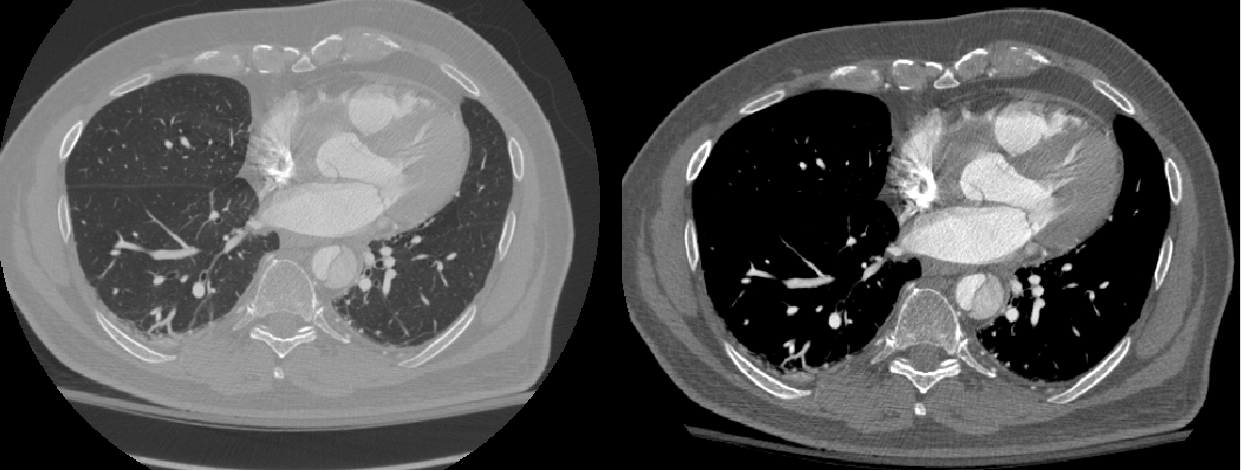
\includegraphics[width=\linewidth]{images/windowing-example}
 \caption{A cardiac CTA in its full range (left) and windowed (right). \cite{radlAVTMulticenterAortic2022a}}
 \label{fig:windowing-example}
 \end{figure}

\subsubsection{Magnetic Resonance Imaging (MRI)}

Much like CT, MRI produces voxel-based images that visualize the insides of an object. The process of obtaining an MRI image can be separated into several steps \cite{groverMagneticResonanceImaging2015}:

\begin{enumerate}
	\item The machine applies a strong magnetic field to the subject. This causes protons in the body to align in the same direction --- parallel to the z-axis.
	\item Next, the machine emits a brief radio frequency pulse, perturbing a small portion of the aligned protons and causing them to deviate from their uniform alignment.
	\item After the pulse is turned off, the protons gradually return back to alignment. As they realign, the movement of their positive charge induces an electric current in a coil inside the MRI machine. In contrast to CT, which gauges the attenuation of X-rays, MRI measures this induced current.
\end{enumerate}

The time to reach the equilibrium state depends on the specific tissue type, so the measured current allows the differentiation of tissues in the image. The equilibrium state is achieved through two independent processes: T1 and T2. T1 measures the time it takes the protons to reach equilibrium longitudinal alignment, while T2 measures the time to regain its equilibrium transverse alignment. Different tissues return to their equilibrium states at varying rates for T1 and T2, enabling two different types of MRI images: T1- or T2-weighted. For example, water exhibits a long T1 time, while fat has a shorter one. This means that in T1-weighted images, fat appears brighter than water, while the opposite is true in T2-weighted images. This can be seen in \figref{fig:t1-t2-example}.

\begin{figure}[!b]
 \centering
 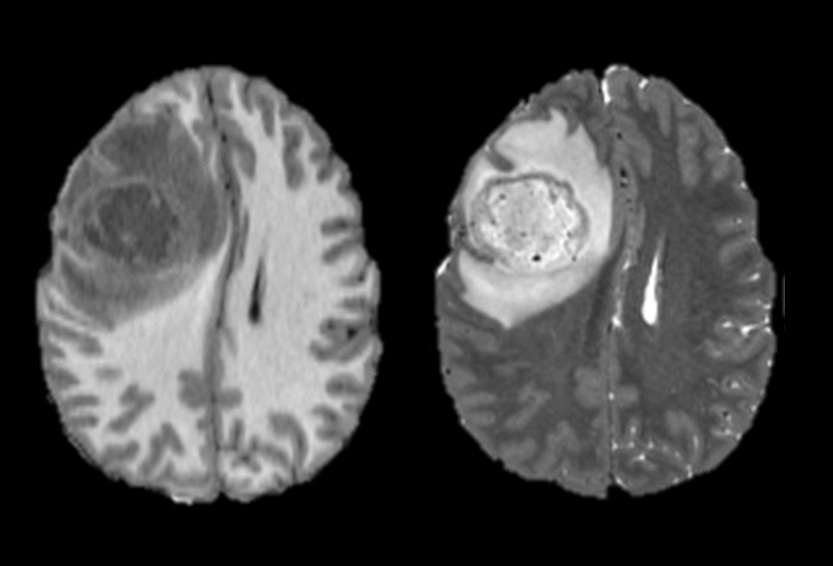
\includegraphics[width=0.65\linewidth]{images/mri-t1-t2-example}
 \caption{An example T1-weighted MRI (left) and a T2-weighted MRI (right) showing a diffuse glioma. \cite{calabreseUniversityCaliforniaSan2022}}
 \label{fig:t1-t2-example}
 \end{figure}
 
 The relative differences in T1 and T2 images make each more suitable for imaging specific tissues \cite{boaventuraT1T2weightedRatio2022}. For instance, T1-weighted images allow for identifying fatty tissue or detecting liver lesions, while T2-weighted images are more effective for identifying white matter lesions and edemas.
  
 The voxels in an MRI, much like a CT, are generally rectangular solids and can be different in width, height, and depth. The image resolution is determined by several factors, including the scanner's field of view, the MRI machine itself, and specific imaging parameters. Generally, increasing resolution leads to higher levels of noise and a longer acquisition time \cite{macovskiNoiseMRI1996}. Consequently, an optimal balance between resolution, noise, and scan time must be found, tailored to the tissue being imaged and the specific diagnostic objective.
 
 MRI has several advantages over CT. For one, MRI usually offers superior contrast, especially when imaging soft tissues \cite{changMagneticResonanceImaging1987}. This has established MRI as the gold standard for a large number of diagnostic procedures. Much like with CT scans, MRI contrast can be further enhanced using contrast agents. Furthermore, as MRI uses magnetic fields instead of ionizing radiation, it poses no radiation-induced risks to patients.
 
However, MRI has its own set of limitations. MRI scans typically take longer than CT scans, which can be uncomfortable for patients, particularly those who are claustrophobic or have mental and cognitive disabilities \cite{thorpeClaustrophobiaMRIRole2008}. MRI is contraindicated for individuals with certain non-removable magnetic objects, like coronary pacemakers and specific implants \cite{steccoPatientSafetyIssues2007}. A notable drawback is the lack of standardization in MRI values across different scans and machines \cite{wahidIntensityStandardizationMethods2021}. Contrary to CT scans, an MRI voxel's intensity is not consistent across different scans and can only be reliably interpreted in relation to adjacent tissue in the same scan.

\subsection{2D Modalities}

3D modalities, while offering a detailed view of a subject, often entail time-consuming and infeasible procedures in common clinical use. 2D modalities such as X-ray and diagnostic ultrasound are often quicker and more readily available. This ease and speed of 2D modalities contribute to the large amount of publicly available datasets in 2D modalities compared to 3D ones. For example, analyzing X-ray images is one of the most active fields in computerized medical image analysis research \cite{nguyen2020vindrcxr, irvinCheXpertLargeChest2019}.

\subsubsection{X-ray imaging}

X-ray imaging, also known as radiography, can be thought of as the 2D equivalent of a CT as it also relies on ionizing radiation \cite{seibertXrayImagingPhysics2004}. To obtain an image, X-rays are emitted on one side of the subject and captured on the opposite side. The intensity of the pixels corresponds to the attenuation of the emitted radiation. Denser materials appear with a higher intensity on the resulting image due to their high attenuation.

When capturing an X-ray image, an expert manually positions the generator. The relative positioning of this generator and the subject directly influences the image's magnification and field of view. If the subject is closer to the detector than the generator, it will appear magnified on the resulting image. Such magnification makes the scale on an X-ray image non-standard and precludes the possibility of making objective length and area measurements.

The expert also determines various parameters that ultimately change the quality and quantity of the X-ray beams. The quality measures the ability of an X-ray to penetrate tissue and is proportional to the X-ray energy level. Quantity, on the other hand, measures the number of photons constituting the beam. A high beam quality is advantageous for imaging denser tissues, like bones, or traversing larger volumes. However, high-quality beams reduce the contrast in soft tissues. Owing to the variability introduced by these parameters, X-ray image intensities lack the uniform standardization found in CT scans. Consequently, there is no standardized unit for gauging X-ray intensity across images.

\subsubsection{Dermatological images (clinical and dermatoscopic)}

The application of deep learning models to dermatology, especially skin lesion analysis, has gained significant momentum. This is driven in part by organizations such as the International Skin Imaging Collaboration (ISIC) which curates large dermatological datasets \cite{rotembergPatientcentricDatasetImages2021}. These datasets consist of two primary types of dermatological images: dermatoscopic and clinical. Clinical images are regular photographs of skin lesions, while dermatoscopic images are captured with a device called a digital epiluminescence dermatoscope. A dermatoscope consists of a camera attached to a magnifying lens with a built-in light source. It allows capturing detailed and magnified images of a skin lesion while filtering out skin reflections.

The primary application of deep learning in dermatological images is for classification, e.g. predicting whether a lesion is benign or not or detecting the type of skin disease. However, by precisely outlining the boundary of a skin lesion, segmentation techniques can yield more consistent and objective descriptors of the lesion, aiding classification algorithms \cite{rotembergPatientcentricDatasetImages2021}.

\subsubsection{Microscopy}

In biomedicine, one of the predominant uses of computer vision is in segmenting, analyzing, and quantifying microscopic images \cite{khanAutoCellSegRobustAutomatic2018}. This covers a broad array of tasks in digital pathology, from identifying cancerous cells and segmenting nuclei to quantifying white blood cell counts.

Publicly available microscopic images of cells are abundant due to how frequently they are captured and that they do not contain any personally identifiable information. However, the large size of these images can present a challenge. Often spanning multiple megapixels, they exceed the capacity of current deep-learning models and machines. Consequently, to make them more manageable, these images are typically divided into smaller patches, downscaled, or processed using a coarse-to-fine approach \cite{jhaInstanceSegmentationWhole2021a}.

As can be seen, both 2D and 3D biomedical images are exceedingly diverse in their appearance, use, technical details, and format. Yet, many segmentation techniques prove versatile enough to be applied across different modalities. In the next section, we will provide a general outline of how image segmentation works, highlighting commonly used methods.

\section{Image Segmentation: From Images to Segmentation Maps}

Image segmentation is the process of categorizing each pixel (or voxel) of an image into one of several predefined classes. Consider a 3-class segmentation scenario for CT images, with classes being liver, liver tumor, and background. Each of these classes is assigned a distinct numeric identifier, termed the \textbf{class label}. For illustration, the labels could be `0', `1', and `2' for the background, liver, and tumor respectively. The segmentation process outputs an image identical in dimensions to the original but with each pixel's value corresponding to the class label of that position in the original image. As an example, pixels corresponding to the liver will all have the value `1'. This resulting image is called a \textbf{segmentation map} since it, like a map, delineates important regions on the original image. 

In medical image segmentation, it is common to extract only a single tissue type against the backdrop, a technique known as \textbf{binary segmentation}. Additionally, multi-class segmentation challenges can be decomposed into multiple binary segmentation tasks, with each class having its individual class-vs-background segmentation map. Therefore, one can frame any segmentation problem as a set of binary segmentation problems.

Mathematically, given a set of $K$ classes, and an input $d$-dimensional image of $N$ channels $I(A)$, $I \in \mathbb{R}^{N}$, $A \in \mathbb{N}^d$ where A is the location of each voxel, the segmentation map $M : \mathbb{N}^d \rightarrow \mathbb{R}^K$ maps each pixel location to a vector of class probabilities:
\begin{equation}
M(A) = (\;\prg{C_1}{I(A)},\; \prg{C_2}{I(A)},\; \cdots\!,\;  \prg{C_{K}}{I(A)}\;),
\end{equation}
where $\operatorname{Pr} (C_i \!\mid\! I(A))$ is the probability that the voxel $I(A)$ contains an object of class $C_i$. Expressed this way, the segmentation map is a $K$-channel image of the same size as $I(A)$. Each channel of the image corresponds to a probability map of finding an object of a given class at a given voxel location. 

In binary segmentation, where $K=2$, the classes can be denoted as $C_1$ for the background and $C_2$ for the target object. Given this, for all voxel locations $A$, the relation $\prg{C_2}{I(A)} = 1 - \prg{C_1}{I(A)}$ holds true. Therefore $M(A)$ simplifies to a scalar value $M(A) = \prg{C_2}{I(A)}$. This representation is very common in medical image segmentation problems such as segmenting organs, cell nuclei, and skin lesions, among others.

Often, the next step in the process is to binarize the segmentation map $M(A)$. Voxels corresponding to the target object are set to `1', while the background is marked as `0'. In such cases, $M(A)$ is frequently termed a \textbf{segmentation mask}. In computer vision, ``mask'' refers to a binary image $M_{01}(A) \in \{0, 1\}$ that hides (masks) regions in another image, resulting in a masked image $I_m(A) = I(A) M_{01}(A)$. Within the context of deep learning-based image segmentation, the terms ``segmentation map'' and ``segmentation mask'' are often used interchangeably.

Having laid the foundation for the mathematical framework of image segmentation, we can now transition to exploring specific segmentation techniques. The next section presents an overview of common segmentation methods, from traditional ones based on heuristics to complex model-based approaches prevalent today.

\subsection{Traditional Image Processing Methods}

Despite the popularity of deep learning, traditional techniques, rooted in fundamental image characteristics, still play a vital role in modern medical image segmentation. Traditional techniques are often used as methods for pre-processing and data augmentation, as well as refining deep learning model outputs. As we will show later in the dissertation, traditional methods can increase the robustness and data efficiency of deep learning-based segmentation models.

Rather than relying on data-intensive training phases, these techniques often operate deterministically, using explicit algorithms that manipulate image characteristics. They directly use image properties such as intensity and texture, combined with heuristic strategies that draw from empirical observations and domain knowledge. Heuristics are best-practice rules derived from previous samples and experiences. For instance, the longest component in the bone intensity range of an X-ray image is usually the femur. These methods provide a clear, interpretable pathway to segmentation.

However, traditional methods are usually developed with a very specific application in mind and are hard to translate to other tasks and domains without significant changes. They are also sensitive to parameter selection and properties of the image such as intensity level. Helpfully, since they do not use a learning component their limitations can be known ahead of time. Their validity can also be confirmed using fewer samples than is the case for learning-based methods.

\subsubsection{Image Thresholding}

Thresholding is a fundamental technique that isolates regions in an image based on a specified range of intensities. In essence, it removes or retains portions of the image where the intensity either falls outside or within a given threshold.

To illustrate the use of thresholding, consider an example of segmenting adipose tissue on a CT scan. As mentioned earlier in this chapter, voxel intensities on CT scans quantify a tissue's X-ray radiation attenuation as measured in Hounsfield units. Typically, fatty tissue lies between -250 HU and -30 HU. Thresholding the entire scan to this range segments fatty tissue from all other tissues on the scan with no need for additional complex models. For preprocessing, Hounsfield unit thresholding is an efficient way to discard irrelevant voxels, allowing the rest of the segmentation process to focus on fewer voxels.

Thresholding can be also used to greatly simplify a model's task using domain knowledge. Take, for instance, the segmentation of epicardial fat, which refers to the fat in proximity to the heart wall. Epicardial fat is sparsely distributed in a complex shape inside the pericardium. Yet, the pericardium itself has a smooth, elliptical shape and is comparatively easy to segment. By first segmenting the pericardium and subsequently thresholding the pericardium region to the fatty tissue range, we can find epicardial fat without having to segment its complex shape directly \cite{bencevicRecentProgressEpicardial2022}.

\subsubsection{Region Growing Techniques}

Region growing is a voxel-based image segmentation method \citep{regionGrowing}. Beginning from a designated seed voxel, the method assesses neighboring pixels in successive steps. If these pixels meet a specified criterion, often related to pixel values or textures, they are integrated into the region. This process continues until all image pixels are assessed. Despite being a straightforward method, region growing is very sensitive to the selected seed point and may struggle with nuanced transitions between regions. This process is shown in \figref{fig:region-growing}.

\begin{figure}[b!]
 \centering
 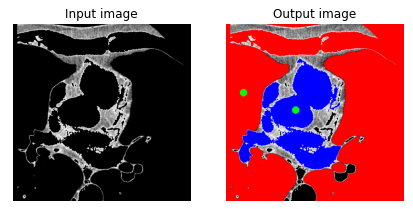
\includegraphics[width=0.7\linewidth]{images/region_growing.png}
 \caption{A demonstration of region growing for delineating the internal and external areas of the pericardium on a CT slice, set to the adipose tissue intensity range. The left image is the original input, and the right image depicts the segmented outcome with the heart exterior in red and the interior in blue. The green dots represent the manually chosen seed points initiating the region-growing technique. \cite{bencevicRecentProgressEpicardial2022}}
 \label{fig:region-growing}
 \end{figure}


\subsubsection{Active Contours or Snakes}

Active contours, often termed ``snakes'', are segmentation methods that employ dynamic curves to outline image parts \citep{Kass1988}. The process involves tightening a preliminary curve around an object iteratively until it conforms to the object's shape. The adaptation is guided by an energy function that evaluates the curve's smoothness and proximity to edges. A practical depiction of active contours is displayed in \figref{fig:active-contour}.

 \begin{figure}[t!]
 \centering
 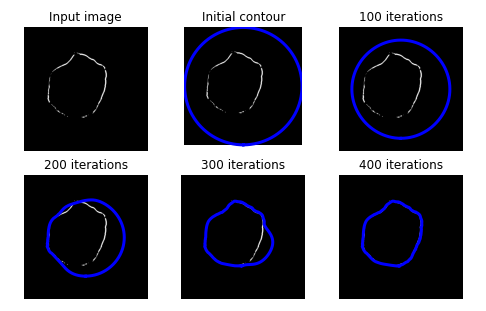
\includegraphics[width=0.65\linewidth]{images/active_contour.png}
 \caption{A demonstration of employing active contours to complete the absent segments of the pericardium line, displayed in white. The contour, illustrated in blue, starts as a complete circle surrounding the image. With every iteration, the contour adapts more closely to the image's shape. \cite{bencevicRecentProgressEpicardial2022}}
 \label{fig:active-contour}
 \end{figure}

\subsubsection{Atlas-Based Segmentation}

Atlas-based methods, differing from contour-based ones, leverage the spatial relationships among identified structures in an image \citep{Rohlfing2005}. First, a template image is selected and an expert creates an atlas (a segmentation map) by manually segmenting and labeling structures in the template image. Due to anatomical variations, multiple representative images are often merged to produce a template image. The atlas can then be employed to segment new images using a registration algorithm. Image registration is an optimization problem where one image, called the moving image, is deformed to best align with a target image according to some scoring function. The scoring function usually uses the distance between heuristic-based landmarks in the target and moving images to determine how well the two images align. In atlas-based segmentation, a new moving image is deformed to be aligned with the template image that was used to construct the atlas. The atlas can then be used as a segmentation map for the moving image, as it is now aligned with the atlas. The atlas-based registration process is illustrated in \figref{fig:registration}.

\begin{figure}[t!]
 \centering
 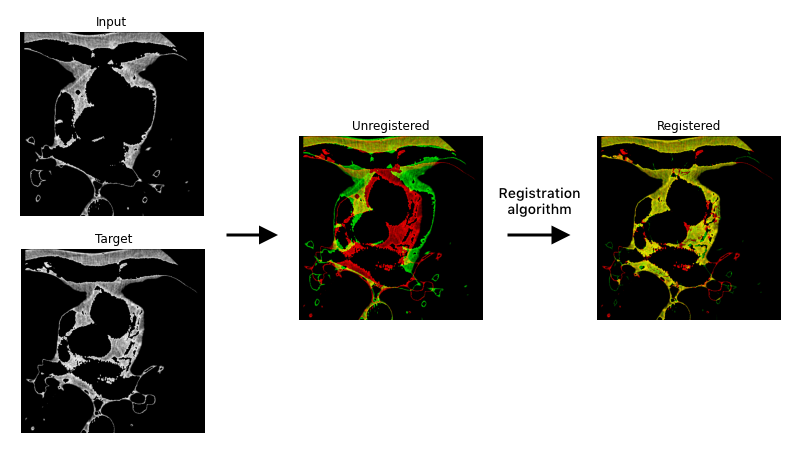
\includegraphics[width=0.7\linewidth]{images/registration.png}
 \caption{A schematic representation of the registration procedure. Initially, input and target images are chosen. Throughout the registration phase, the input image (shown in green) undergoes deformation to align with the fixed target image (shown in red). \cite{bencevicRecentProgressEpicardial2022}}
 \label{fig:registration}
 \end{figure}

A disadvantage of this approach is that the process can lead to a complete failure to segment the image if the target and moving images are too dissimilar. Therefore, atlas-based segmentation has fallen out of favor due to the emergence of deep learning-based methods. However, recently there has been significant progress in image registration and atlas-based segmentation using deep learning-based techniques \cite{sinclairAtlasISTNJointSegmentation2022a}. These approaches offer good potential for merging traditional and newer approaches will be discussed later in the chapter.

\subsection{Machine Learning}

While deep learning generally falls within the machine learning umbrella term, in this dissertation the term ``machine learning'' will be used to refer to techniques that are not based on deep neural networks. This encompasses methods such as support vector machines, random forests, and other statistical learning techniques that rely on manually engineered image features.

In this context, image segmentation can be viewed as a voxel-wise classification problem expressed as
\begin{equation}
H(x; \theta) = (\;\operatorname{Pr}(C_0\!\mid\!x),\; \operatorname{Pr}(C_1\!\mid\!x),\; \cdots,\; \operatorname{Pr}(C_{K-1}\!\mid\!x)\;),
\end{equation}
where $H$ is a classification function parameterized by $\theta$, which maps an input vector $x$ of voxel-level features to the probability that the voxel contains the class $C_i$. The features are manually constructed based on domain knowledge and represent each pixel and its surrounding region. Commonly, these include the pixel's intensity, mean intensity of the area, image moments, and other information deemed relevant for the classification. The classifier is trained to minimize a predefined loss function by feeding each pixel's features to the classifier and comparing the output to the ground truth output. This is presented visually in \figref{fig:machine-learning}.

\begin{figure}[t!]
 \centering
 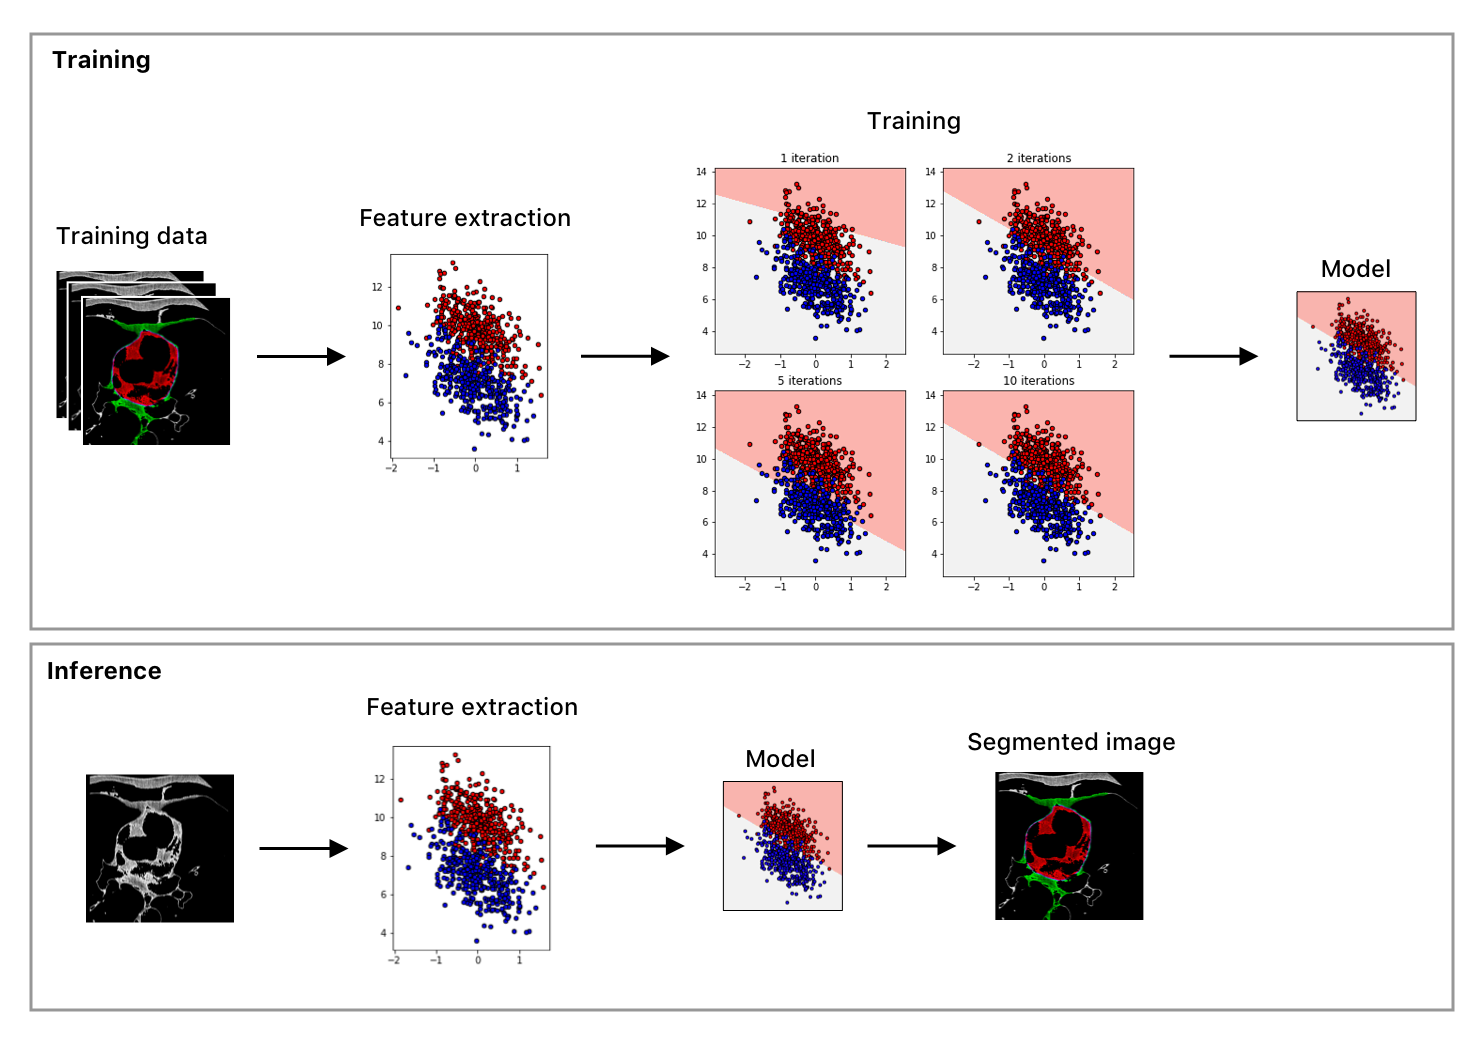
\includegraphics[width=\linewidth]{images/machine_learning.png}
 \caption{A schematic of a supervised linear classifier in a machine learning workflow. The upper section illustrates the training phase. Here, features are color-coded according to their known class from training data, depicted in red and blue. The parameters of the decision boundary, which demarcates the zones of the two classes (highlighted in light red and grey), are determined during training. The lower part of the diagram depicts the inference stage. In this phase, features are extracted from new images, and the trained model is employed to classify each pixel in the image. \cite{bencevicRecentProgressEpicardial2022}}
 \label{fig:machine-learning}
 \end{figure}

Another common approach is to divide the image into smaller patches and then employ a machine learning classifier to categorize each patch into one of the predefined $K$ classes. The classifications are then fused together to form a segmentation map. Both patch- and voxel-based machine learning approaches can be more data efficient than deep learning-based approaches \cite{bencevicRecentProgressEpicardial2022}, but they often lack the ability to model complex features and dependencies. 

It is clear that these traditional techniques have inspired and paved the way for more complex deep learning methods --- while still playing a vital role as parts of segmentation pipelines today. In the next section, we will provide an overview of how deep learning builds on traditional machine learning to achieve more powerful models that can segment very complex regions.

\pagebreak

\section{Deep Learning-Based Segmentation Methods}

Machine learning encompasses a broad range of techniques for building statistical models, which includes deep learning --- a subset of machine learning that focuses on using artificial neural networks. Artificial neural networks consist of simple nodes called \textbf{neurons}. Each neuron is a non-linear function of the sum of its inputs. This non-linear function is called the \textbf{activation function}. The neurons are all arranged in a graph where the outputs of one set of neurons are connected to the input of another set of neurons. Each connection has an associated \textbf{weight} and \textbf{bias} parameter. The value on the connection is multiplied by the weight and the bias is added before it is fed into the subsequent neuron. The exact configuration of the graph, including the number of neurons and how they are connected, is determined by hand and is referred to as the \textbf{neural network architecture}. Typically neurons are arranged into \textbf{layers}, where neurons of one layer connect only to the next layer. Current deep-learning networks usually have between ten and 100 layers. A typical neural network architecture can be seen in \figref{fig:nn-typical}.

\begin{figure}[t!]
 \centering
 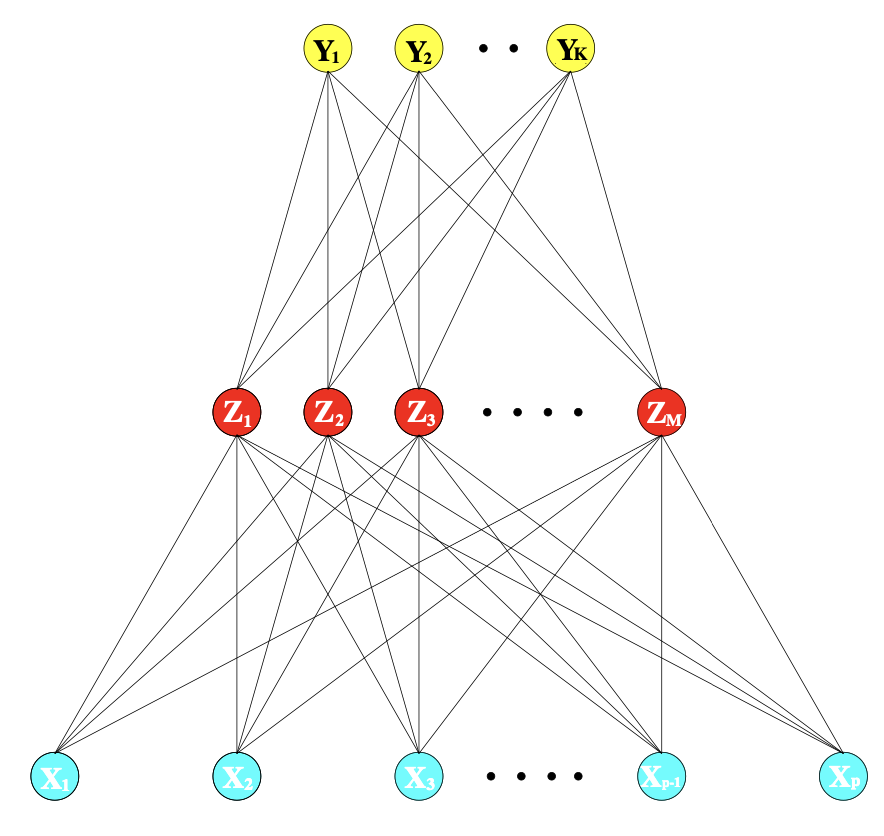
\includegraphics[width=0.5\linewidth]{images/nn-typical}
 \caption{A small neural network with three layers, wherein each layer is connected to every neuron in the next layer. \cite{hastieElementsStatisticalLearning2009}}
 \label{fig:nn-typical}
 \end{figure}

Mathematically, a neuron is a function that maps some input vector to a scalar value. First, the dot product between the input vector $x = [x_0\; x_1\; \cdots\; x_{n - 1}]$ and the weights column vector $w$ is calculated and added with the bias vector $b$:
\begin{equation}
z(x;w, b) =
\begin{bmatrix}
x_0 & x_1 & \cdots & x_{n - 1}
\end{bmatrix}
\begin{bmatrix}
w_0\\
w_1\\
\cdots\\
w_{n-1}
\end{bmatrix}
+
\begin{bmatrix}
b_0 & b_1 & \cdots & b_{n - 1}
\end{bmatrix}.
\end{equation}

Then, all of the inputs are summed and the neuron output is produced using the activation function $g$:
\begin{equation}
f(x;w,b) = g\left(\sum_{i=0}^{n - 1} z(x;w,b)_i\right).
\end{equation}
The parameters $b$ and $w$ associated with each neuron can be consolidated into a large matrix, denoted as $\theta$. This matrix is called the \textbf{parameters of the network}. Current deep learning networks usually have multiple millions of parameters.

One example of an activation function is the rectified linear unit (ReLU) function:
\begin{equation}
ReLU(x) = 
    \begin{cases}
        x, & \text{if } x > 0,\\
        0, & \text{otherwise.}\\
    \end{cases}.
\end{equation}
ReLU can be seen as a simple thresholding function that sets all negative values to zero. Despite its simplicity, ReLU is one of the most prevalent activation functions in neural networks.

\subsection{Neural Network Training, Validation and Testing}

Initially, the parameters of a neural network are often initialized with random values. These values are then fine-tuned during a procedure called \textbf{training}, which iteratively adjusts the parameters to minimize a \textbf{loss function}. The loss function measures how well the network is performing its task by comparing its output to known correct values. For example, in image segmentation, the loss function would measure the similarity between the network's segmentation map and a hand-labeled counterpart. Through a process called \textbf{backpropagation}, each parameter is updated in the direction that will decrease the loss. This is repeated multiple times for each image in a \textbf{training dataset}.

However, there is a caveat. The training dataset, much like any statistical data, is a sampling of the ``real world'' data from some unknown distribution. Depending on the size and quality of the dataset, it is possible that the training dataset does not represent the true distribution of the data. Moreover, the network can learn to produce correct solutions for each training image individually instead of learning general patterns in the data. This is called \textbf{overfitting} --- the model excels on the training data but fails on unseen data. To detect and mitigate this, two additional datasets are introduced: the \textbf{validation} and \textbf{test} datasets.

The \textbf{validation dataset} serves a critical role during model development. After training, the model is assessed using this dataset to inform decisions about its architecture, preprocessing, and other facets. During the development cycle, the network is constantly modified and re-evaluated on the validation dataset. Since adjustments to the model are based on its performance on the validation dataset, there's a risk of inadvertently tailoring the model to the specific distribution of the validation data. To counteract this potential bias, a \textbf{test dataset} (often termed a hold-out dataset) is used. This dataset is reserved exclusively for a final evaluation, offering the least biased estimate of the model's real-world performance.

The training, validation, and testing datasets are created before the model development process. Usually, they are sampled randomly from a larger dataset with ratios such as 80\%, 10\% and 10\% for the training, validation, and testing datasets, respectively. 

In the next chapter, we will further discuss overfitting in neural networks. For now, we will move on to describing neural network architectures in more detail.

\subsection{Encoders and Decoders}

Machine and deep learning-based segmentation methods can be conceptualized as a two-stage process. The first stage, termed the \textbf{encoder} stage, is a function $En : \mathbb{R}^{D \times C} \rightarrow \mathbb{R}^{n \times m \times d}$. In other words, a $D$-dimensional image with $C$ channels is mapped to a tensor commonly referred to as a feature map. This feature map has an arbitrary size and depth determined by the network architecture. The encoder effectively compresses the image by distilling salient information into a smaller representation, the feature map. In deep learning parlance sometimes this is referred to as the \textbf{backbone} of the network.

The output of the encoder then goes to the second stage called the \textbf{decoder} or the \textbf{head}. The decoder is a function $De : \mathbb{R}^{n \times m \times d} \rightarrow \mathbb{R}^{D \times K}$ that maps a given feature map into a segmentation map. 

Given an image $I(A)$, the segmentation process can then be written as
\begin{equation}
M(A) = (En(\theta_{En}) \circ De(\theta_{De}))(I(A)),
\end{equation}
where $En$ and $De$ are functions parameterized by a $\theta_{En}$ and $\theta_{De}$, respectively. In conventional machine learning, $En$ is not a trainable function. Instead, $\theta_{En}$ consists of hand-selected parameters to extract pre-selected features from the image. The value of $\theta_{De}$, on the other hand, is determined by minimizing a loss function. In deep learning, both $\theta_{En}$ and $\theta_{De}$ are determined by minimizing a loss function.

Thus, the difference between traditional machine learning and deep learning is in the encoder stage. Deep learning utilizes neural networks to define features, whereas traditional machine learning uses handcrafted functions.

The separation of segmentation models into encoder and decoder stages is a crucial aspect of current research in deep learning. This separation allows for independent improvement of both stages and an easy combination of different encoders and decoders. For instance, a classification and segmentation network could use the same encoder architecture. While the classifier would utilize a simpler decoder to map input features to a class probability vector, the segmentation model would employ a more complex decoder to produce a segmentation map. However, both models would use the exact same encoder. In fact, there are models such as Mask R-CNN \cite{heMaskRCNN2017b} that use two parallel decoders, one for segmentation and another for object detection, both connected to the same encoder. Throughout the rest of this thesis, when describing neural network architectures, we will describe them in terms of their encoder and decoder and how the two are connected.

\subsection{Convolutional Neural Networks}

Convolutional neural networks have profoundly impacted computer vision, establishing deep learning as the prevailing approach for complex computer vision tasks. The foundational element of a CNN is its convolutional layer, which uses a convolution-like operation in place of the conventional neurons mentioned earlier in this chapter.

\subsubsection{Convolution}

\begin{figure}[b!]
 \centering
 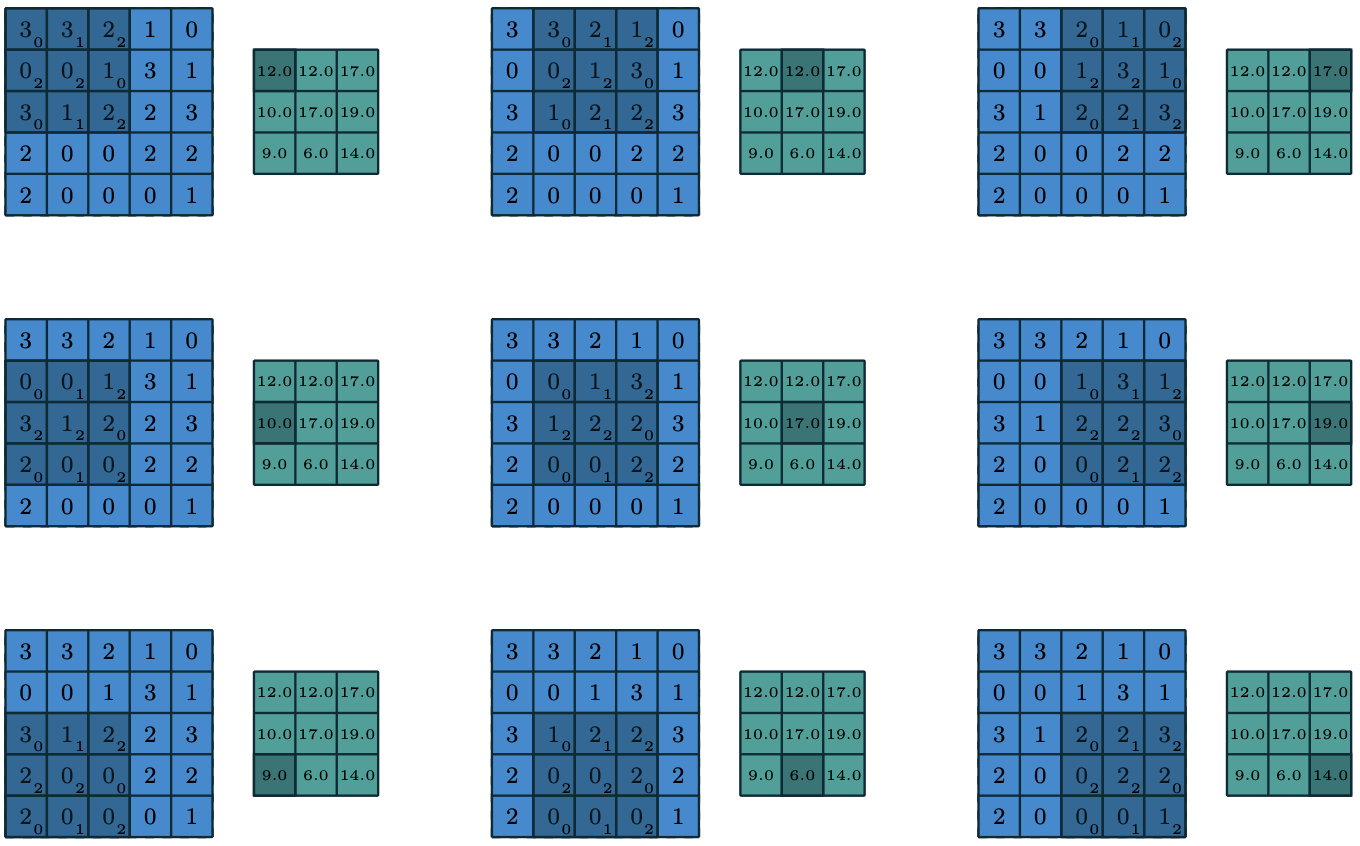
\includegraphics[width=\linewidth]{images/convolution-explainer.png}
 \caption{A visual depiction of a convolution procedure step-by-step. In each step, the kernel slides over the image (shown in blue). The overlapping elements between the kernel and the image are multiplied and then summed to produce a value in the resultant image (shown in green). \cite{dumoulinGuideConvolutionArithmetic2018}}
 \label{fig:convolution-explanation}
 \end{figure}

Generally, convolution is a mathematical operation between two functions. In the context of this thesis, however, we will focus on discrete 2D convolution between two square images, as that is most relevant for image segmentation. Convolution is denoted as $I(A) \star k(B)$ where $I(A)$ is an image $I(A) \in \mathbb{R}^{W \times H}$ and $k(B)$ is a matrix $k(B) \in \mathbb{R}^{w \times h}$ indexed by locations $B \in \mathbb{N}^2$ for called the \textbf{convolutional kernel}. At position $A = (a_x, a_y)$, the convolution operation is defined as
\begin{equation}
(I \star k)(a_x, a_y) = \sum_{j=1}^{h} \sum_{i=1}^{w} I[a_x - i, a_y - j] k[i, j].
\end{equation}

Explained differently, the resulting image is produced by sliding the kernel over the input image pixel by pixel. At each pixel location, values where the kernel and the image overlap are multiplied, and all of the products are summed together to form the corresponding pixel's value in the output image. This is shown visually in \figref{fig:convolution-explanation}.

While mathematically a simple operation, convolution is exceedingly powerful and can produce almost endless transformations of an image. It is most commonly used for filtering --- a convolution can elegantly find patterns in the image and increase their intensity in the image. One such example is the convolution with a kernel called the Prewitt operator:
\begin{equation}
I_y(A) = I(A) \star \begin{bmatrix}
-1 & 0 & 1\\
-1 & 0 & 1\\
-1 & 0 & 1\\
\end{bmatrix}.
\end{equation}
When convolved with this kernel, the resulting image has high-intensity pixels in regions where vertical edges are present, and low intensity everywhere else. This can be seen in \figref{fig:prewitt-example}.

\begin{figure}[b!]
 \centering
 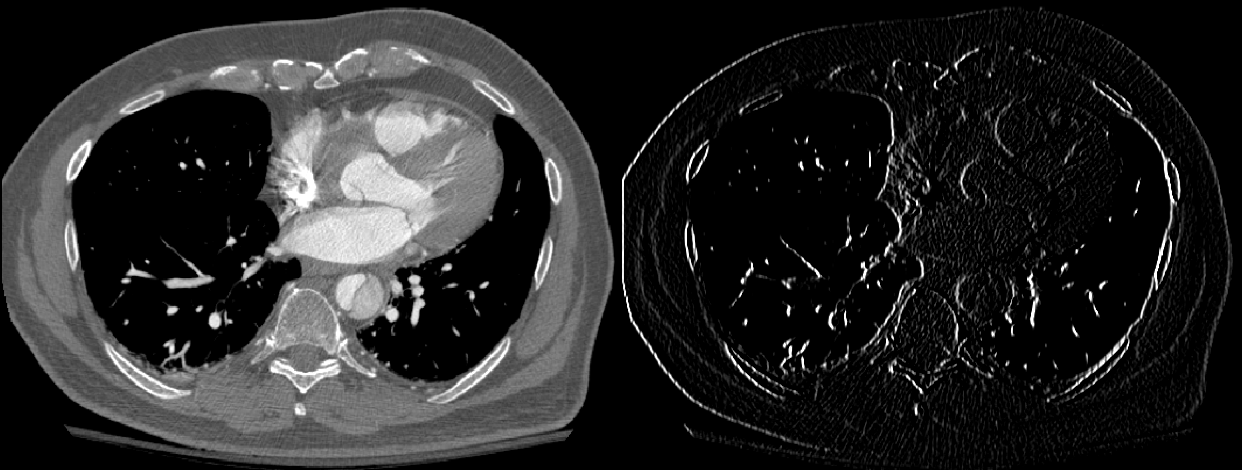
\includegraphics[width=\linewidth]{images/prewitt-example.png}
 \caption{An example of an input image (left) convolved with the Prewitt operator (right). Note that vertical edges are accentuated in the convolution result.}
 \label{fig:prewitt-example}
 \end{figure}

Vertical edges necessarily have to have a large jump in values going from left to right or right to left. Otherwise, there would be no perceptible edge. This kernel takes advantage of that fact to accentuate parts of the image where there is such a jump. It does this by replacing each pixel with the difference between the pixels on its left and its right.

This process happens as follows. For each pixel of the input image, the kernel is placed such that it is centered on that pixel. This means that the values of the pixel as well as its neighbors above and below are all multiplied by zero. The neighbors on the left are multiplied by -1, and the ones on the right are multiplied by 1. Summed together, the result represents the sum of the values on the right of the pixel, minus the sum of the values on the left.

To illustrate this, let us consider $1 \times 3$ region of the image where no vertical edges are present:

\[
\begin{bmatrix}
128 & 130 & 136\\
\end{bmatrix}
\star
\begin{bmatrix}
-1 & 0 & 1\\
-1 & 0 & 1\\
-1 & 0 & 1\\
\end{bmatrix}
=
\sum_{i,j}
\begin{bmatrix}
-1 \times 0 + 0 \times 128 + 1 \times 130\\ 
-1 \times 128 + 0 \times 130 + 1 \times 136\\
-1 \times 130 + 0 \times 136 + 1 \times 0\\
\end{bmatrix}
= 8
\]

This section of the image does not contain a vertical edge, so the convolution result is a relatively low value. In a standard image with values in $[0, 255)$, 8 would appear almost completely black.

However, consider some section of the image where a vertical edge is indeed present:

\[
\begin{bmatrix}
63 & 66 & 132\\
\end{bmatrix}
\star
\begin{bmatrix}
-1 & 0 & 1\\
-1 & 0 & 1\\
-1 & 0 & 1\\
\end{bmatrix}
=
\sum_{i,j}
\begin{bmatrix}
-1 \times 0 + 0 \times 64 + 1 \times 66\\ 
-1 \times 64 + 0 \times 66 + 1 \times 132\\
-1 \times 66 + 0 \times 132 + 1 \times 0\\
\end{bmatrix}
= 68
\]

The value is now much larger due to the difference between the left and right sides of the image. This example demonstrates how a relatively simple kernel can capture complex features of an image.

Beyond edge detection, there are many commonly used convolution kernels to perform tasks such as blurring, sharpening, or denoising images. A CNN can leverage the power of the convolution by stringing together sequences of intricate kernels to match complex patterns in the image.

\subsubsection{Convolutional Layers}

A CNN operates by passing an image through a sequence of convolutions. The output from one convolution serves as the input for the next. Interspersed between these convolutions are non-linear transformations of the outputs. This layered approach enables the network to successively find more and more intricate features by combining simpler ones. For instance, combining edges into corners, corners into shapes, and ultimately detecting objects from shapes. The addition of non-linearity drastically increases the complexity of features the network is able to detect and combine.

More technically, in a CNN, convolutional layers are connected to one another in a similar fashion to neurons in a regular neural network. Each layer performs a set number of convolutions, denoted by $n$. The results are stored in an $n$-channeled \textbf{feature map}. Each channel corresponds to a convolution with a distinct kernel. Hence, a convolutional layer contains $n$ unique kernels. The values of the kernels are the parameters of the layer, optimized during training to minimize a loss function like weights and biases of standard neurons. Finally, a convolutional layer also applies a non-linear activation function to the resulting feature map.

It is worth noting that the operation within a convolutional layer differs from a standard 2D discrete convolution. Here, both the kernel and the input are three-dimensional and have the same depth, but the kernel is usually much smaller in width and height. Since the kernel has the same width as the input, during the operation the kernel only slides along the width and height dimensions. The output of each sliding window step is still a single scalar since all overlapping elements in the sliding window volume are multiplied and summed together. This means that the output of the whole operation is a two-dimensional image. This is visualized in \figref{fig:cnn-conv-explained}.

\begin{figure}[t!]
 \centering
 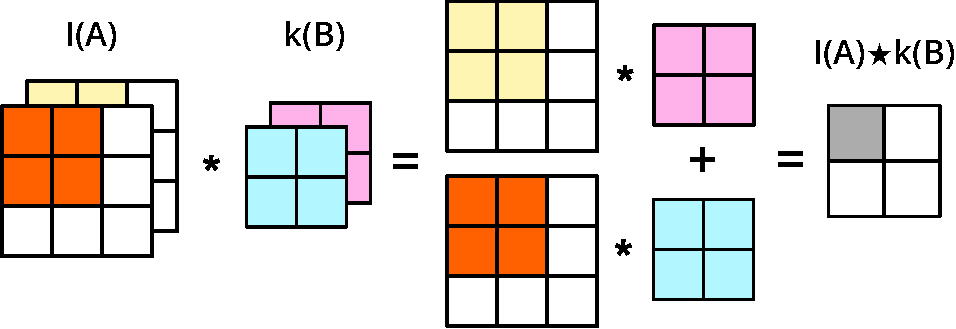
\includegraphics[width=0.8\linewidth]{images/cnn-operation-explained}
 \caption{A view of one step of a single convolution operation inside a CNN layer. The layer performs multiple convolutions, each with a different kernel that has an equal number of channels as the input image. In each step, the whole kernel slides over the width and height of the image, and the overlapping channels are multiplied together and summed to produce a single output value. The output of the convolution is one channel of a $n$-channel image where $n$ is the number of different kernels in the layer.}
 \label{fig:cnn-conv-explained}
 \end{figure}
 
\subsubsection{Pooling Layers}

Most CNN-based encoders follow a pattern of gradually reducing the width and height of the feature maps while increasing their depth. Depth is increased by giving each successive convolutional layer more kernels. Since each channel represents the result of a convolution with a specific kernel, having more kernels directly increases the output depth. To reduce the width and height, \textbf{pooling layers} are employed. These layers downsample the image, often by averaging pixel values within a defined neighborhood. This downsampling serves dual purposes in a CNN. Firstly, it compresses the image by gradually removing spatial information and retaining relevant semantic information. Secondly, the network is gradually able to build up large complex features by combining small general features. Such an architecture is shown in \figref{fig:cnn-encoder-achitecture}.

\begin{figure}[b!]
 \centering
 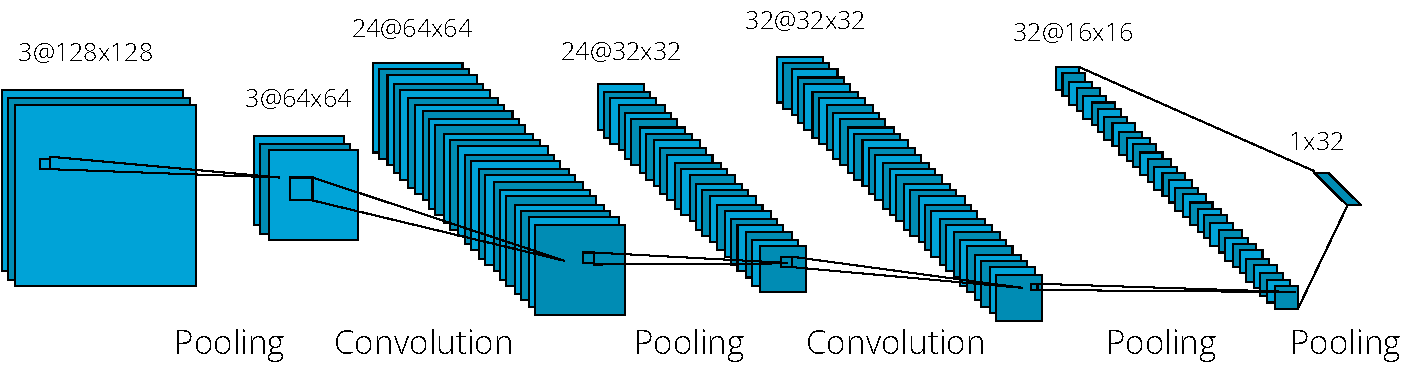
\includegraphics[width=\linewidth]{images/cnn_encoder_example.pdf}
 \caption{A typical architecture of a CNN encoder. The encoder consists of consecutive convolutional and pooling layers that gradually increase the feature map depth and decrease its width and height. The result is a map of features that tells the decoder what features are on the image but does not provide much spatial information about the location of those features. \cite{lecunGradientbasedLearningApplied1998}}
 \label{fig:cnn-encoder-achitecture}
 \end{figure}

To illustrate this, consider a contrived example of a CNN encoder trained to detect grapes on a vine. The first few layers might focus on simple operations such as edge detection, requiring a large amount of spatial information. The next layer could use the edge information to detect circles. This layer does not need as much spatial detail since the edges are already identified. A third layer might then combine the locations of the circles to detect a cluster of grapes. By this stage, the spatial information is even less important, with the overall arrangement of circles being the primary focus.

A convolutional decoder essentially reverses the encoder process. Instead of adding channels, a convolutional decoder successively removes channels up to and upsamples the image. By the end, the output matches the input image's width and height, and the number of output channels equals the number of classes.

One way in which upsampling is implemented in a convolutional decoder is with a \textbf{transposed convolutional layer}. These layers are very common in segmentation neural networks and allow for dynamic, learned upsampling of the image. Regular convolutions cannot increase the image dimension width and height. To overcome this, a transposed convolution produces an output matrix for each step of the sliding window process, instead of just a scalar value. For instance, a transposed convolution with a $2 \times 2$ kernel produces 4 new values for each pixel in the input image. This is done by performing scalar multiplication of the whole kernel and the pixel it is sliding over during each sliding window step. All of the sliding window results are joined as a grid to form a final, larger, image.

To better understand this, consider an example of upscaling a $2 \times 2$ 2D input image $m$ with a $2 \times 2$ kernel $k$. The transposed convolution can be calculated as follows:

\begin{align*}
m \star^T k = & 
\begin{bmatrix}
m_{11}k_{11} & m_{11}k_{12} & 0\\
m_{11}k_{21} & m_{11}k_{22} & 0\\
0 & 0 & 0\\
\end{bmatrix}
+
\begin{bmatrix}
0 & m_{12}k_{11} & m_{12}k_{12}\\
0 & m_{12}k_{21} & m_{12}k_{22}\\
0 & 0 & 0\\
\end{bmatrix}
+\\
&
\begin{bmatrix}
0 & 0 & 0\\
m_{21}k_{11} & m_{21}k_{12} & 0\\
m_{21}k_{21} & m_{21}k_{22} & 0\\
\end{bmatrix}
+
\begin{bmatrix}
0 & 0 & 0\\
0 & m_{22}k_{11} & m_{22}k_{12}\\
0 & m_{22}k_{21} & m_{22}k_{22}\\
\end{bmatrix}
\end{align*}

This method can be similarly applied to images and kernels of any size. While transposed convolution is often referred to as \textit{deconvolution}, in this thesis, we will avoid using the term to prevent confusion with the meaning of deconvolution outside of the context of deep learning.

Segmentation models that use only convolutional and pooling layers are called \textbf{fully convolutional models} and are one of the most widely used types of models for medical image segmentation. In the following section, we will describe these and other commonly used CNN architectures in medical image segmentation.

\section{CNN Architectures for Medical Image Segmentation}

Deep learning's application in medical image segmentation has predominantly seen the use of convolutional neural networks. This field has witnessed a rapid evolution, giving rise to a diverse range of architectures. While some of these architectures were initially designed for general image classification and segmentation tasks, others have been specifically tailored to overcome challenges specific to medical imaging. In this section, we will highlight the most influential CNN architectures that have shaped medical image segmentation, presented in their chronological development.

\subsection{Fully Convolutional Network (FCN)}

The fully convolutional network (FCN), one of the more straightforward contemporary CNN architectures for image segmentation, was introduced in \cite{long2015fully}. As mentioned earlier, convolutional encoders gradually downsample the image while increasing the number of channels in the feature maps. There is then a need to reverse the process and decode the features into an image of equal width and height as the original input image. FCN achieves this using convolutional layers and upscaling.

In FCN, the output of the encoder is interpreted as a coarse heatmap of detected features. An output segmentation map needs to be constructed based on these features and have a number of channels equal to the number of classes. FCN does this by using a convolutional layer with $1 \times 1$ kernels --- one kernel for each class. The resulting convolutions combine the features depth-wise to form a class prediction for each location of the image. However, the resulting segmentation map has a very low spatial resolution. To be useful, it needs to be upsampled using transposed convolution to the original image resolution.

As noted earlier, the encoder's output feature map is only a rudimentary representation of spatial details. To inject additional spatial information into the final segmentation, FCN combines predictions from multiple encoder layers to form the final prediction. This is done by upsampling $1 \times 1$ convolution results from different encoder layers to a uniform size and summing them together. The composite prediction is then upsampled to the original image resolution. This process is shown in \figref{fig:fcn-arch}. 

\begin{figure}[t!]
 \centering
 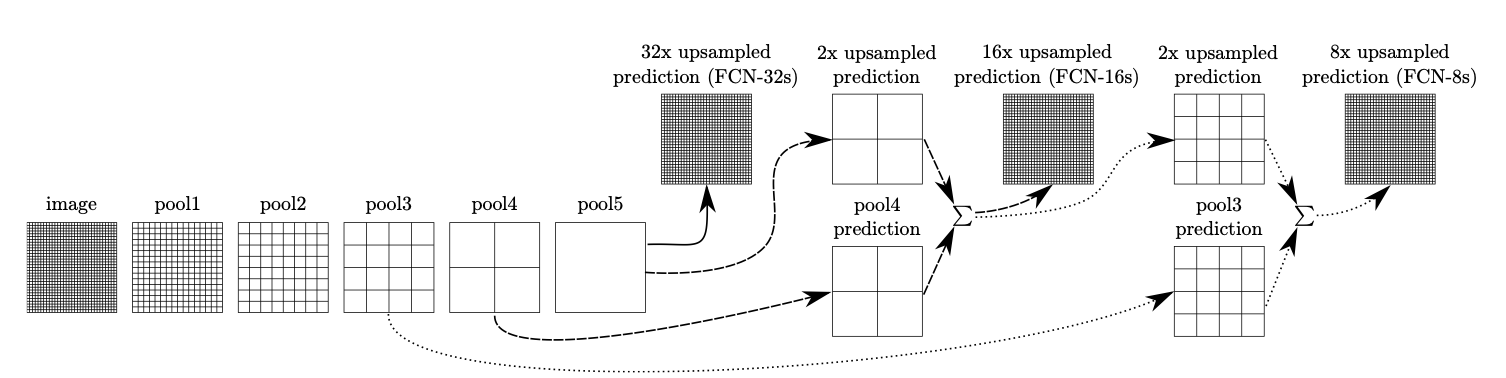
\includegraphics[width=\linewidth]{images/fcn-arch}
 \caption{A diagram of how FCN forms predictions based on the output of different encoder layers. Encoder layers are shown on the left and the grid represents the coarseness of the feature map. The maps are combined at three different levels to produce three predictions. Each prediction is compared with the ground truth during training, but for inference only the 8x upsampled prediction is used. \cite{long2015fully}}
 \label{fig:fcn-arch}
 \end{figure}
 
 \subsection{U-Net and Its Variants}

U-Net \cite{ronnebergerUNetConvolutionalNetworks2015d} is one of the most influential and commonly used architectures in medical image segmentation. Aside from being a standard baseline model, a well-tuned U-Net network with data preprocessing has reached state-of-the-art performance in various segmentation challenges across different domains and modalities \cite{isenseeNnUNetSelfconfiguringMethod2021}.

At its core, U-Net follows a straightforward architectural pattern, comprised of a fully convolutional encoder and decoder with only convolutional and pooling layers. The encoder and decoder have a symmetrical structure: the encoder gradually decreases the width and height of the feature maps while increasing the number of channels, while the decoder does the opposite using upsampling or transposed convolutions. While FCN uses only one $1 \times 1$ convolutional layer and upsampling to form a prediction, U-Net uses a sequence of several convolutional and upsampling layers to gradually build a segmentation map. This progressive structure allows U-Net to produce more detailed feature maps.

Earlier we mentioned that spatial information is important for the precise localization of the features. Like FCN, U-Net also uses the outputs of different encoder layers to maintain spatial information in the decoder but does so in a different way. In U-Net, the output of every encoder layer is added to the input of its corresponding decoder layer on the other side of the network. This gives each decoder layer concurrent access to information about which features are on the image and where they are located. U-Net's architecture can be seen in \figref{fig:unet-arch}.

\begin{figure}[t!]
 \centering
 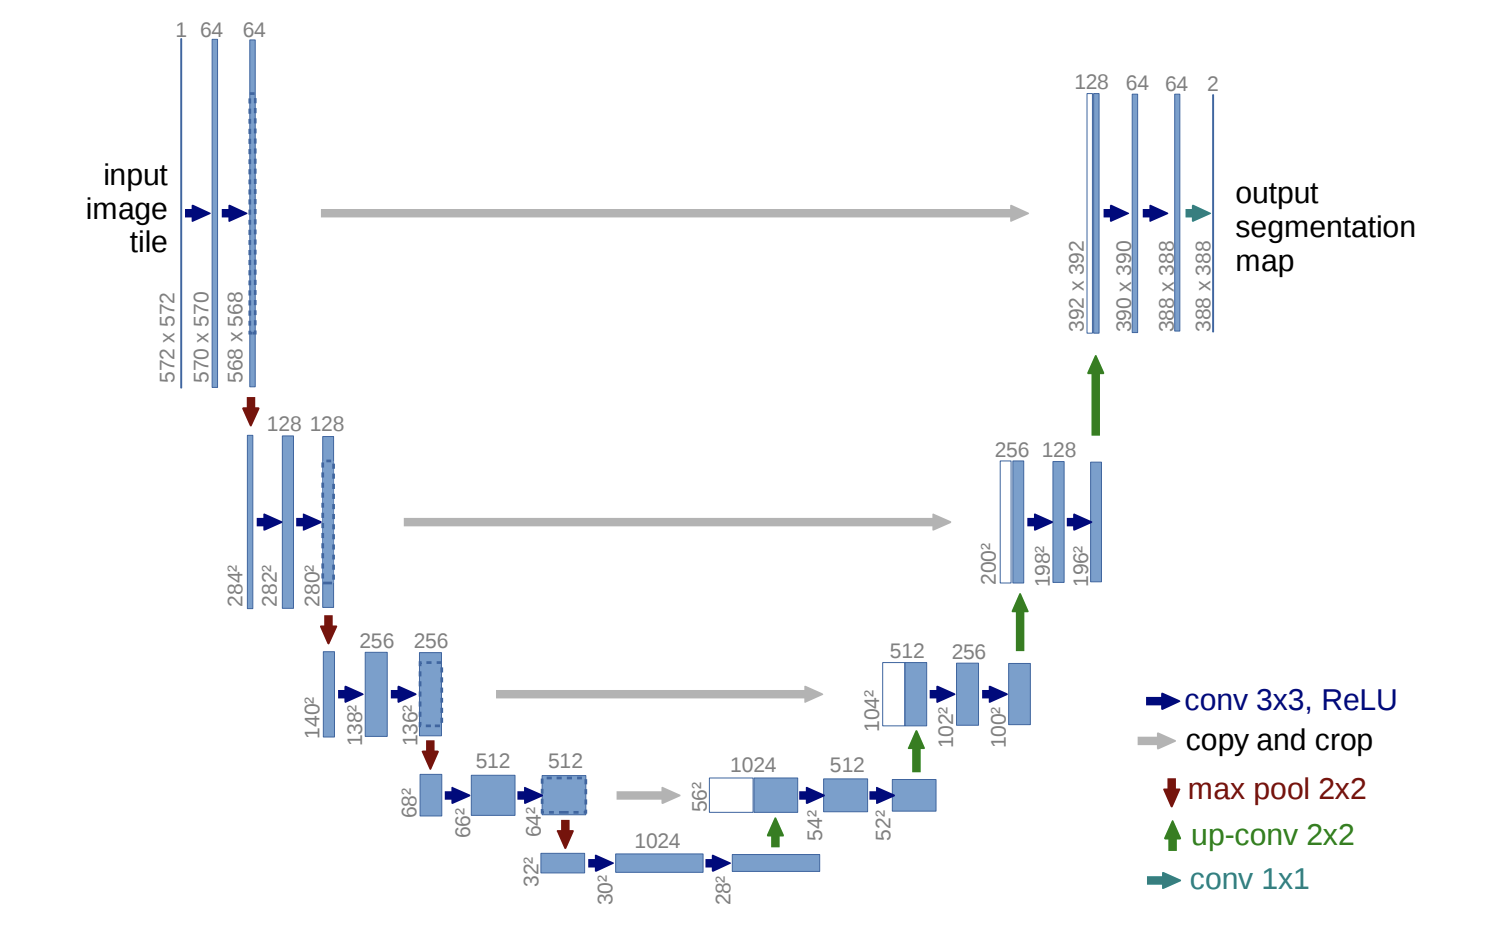
\includegraphics[width=0.8\linewidth]{images/unet-arch}
 \caption{A diagram of the U-Net model. The output of each layer of the encoder is concatenated to the input of its corresponding layer in the decoder. \cite{ronnebergerUNetConvolutionalNetworks2015d}}
 \label{fig:unet-arch}
 \end{figure}

Because of its symmetrical structure and skip connections, U-Net is often visualized in the shape of the letter U, giving it its name. U-Net is only one of a class of networks that are sometimes called U-shaped networks. Aside from being a state-of-the-art architecture for medical image segmentation, U-Net is also widely used as a component of influential deep learning models in other domains such as image generation \cite{rombach2021highresolution} and registration \cite{sinclairAtlasISTNJointSegmentation2022a}.

\subsubsection{nnU-Net}

U-Net is a powerful baseline model that can be carefully tuned using various heuristics and combined with beneficial data preprocessing to achieve state-of-the-art results, even when compared to much more complex models. However, tuning the parameters of the model and preprocessing is a laborious process that requires experise and empirical research. nnU-Net \cite{isenseeNnUNetSelfconfiguringMethod2021} aims to automate this tuning process by producing an optimal data pre- and postprocessing pipeline and a U-Net-based architecture for a given dataset. This is achieved through a set of heuristics, rules, and optimization techniques.

The nnU-Net framework begins by calculating key parameters of the data distribution, such as intensity distribution and median image size. Based on these parameters, a set of predefined rules determine the network's architecture and training strategy, including the number of layers, training parameters, and preprocessing approach.

Using the determined parameters, nnU-Net trains three models: one using 2D slices of the data, another using the entire 3D volume, and the third using a cropped 3D region of interest. During inference, outputs from these models are combined through preprocessing to form an ensemble prediction, enhancing the overall accuracy and robustness of the segmentation. This process is shown in \figref{fig:nnunet-arch}.

\begin{figure}[t!]
 \centering
 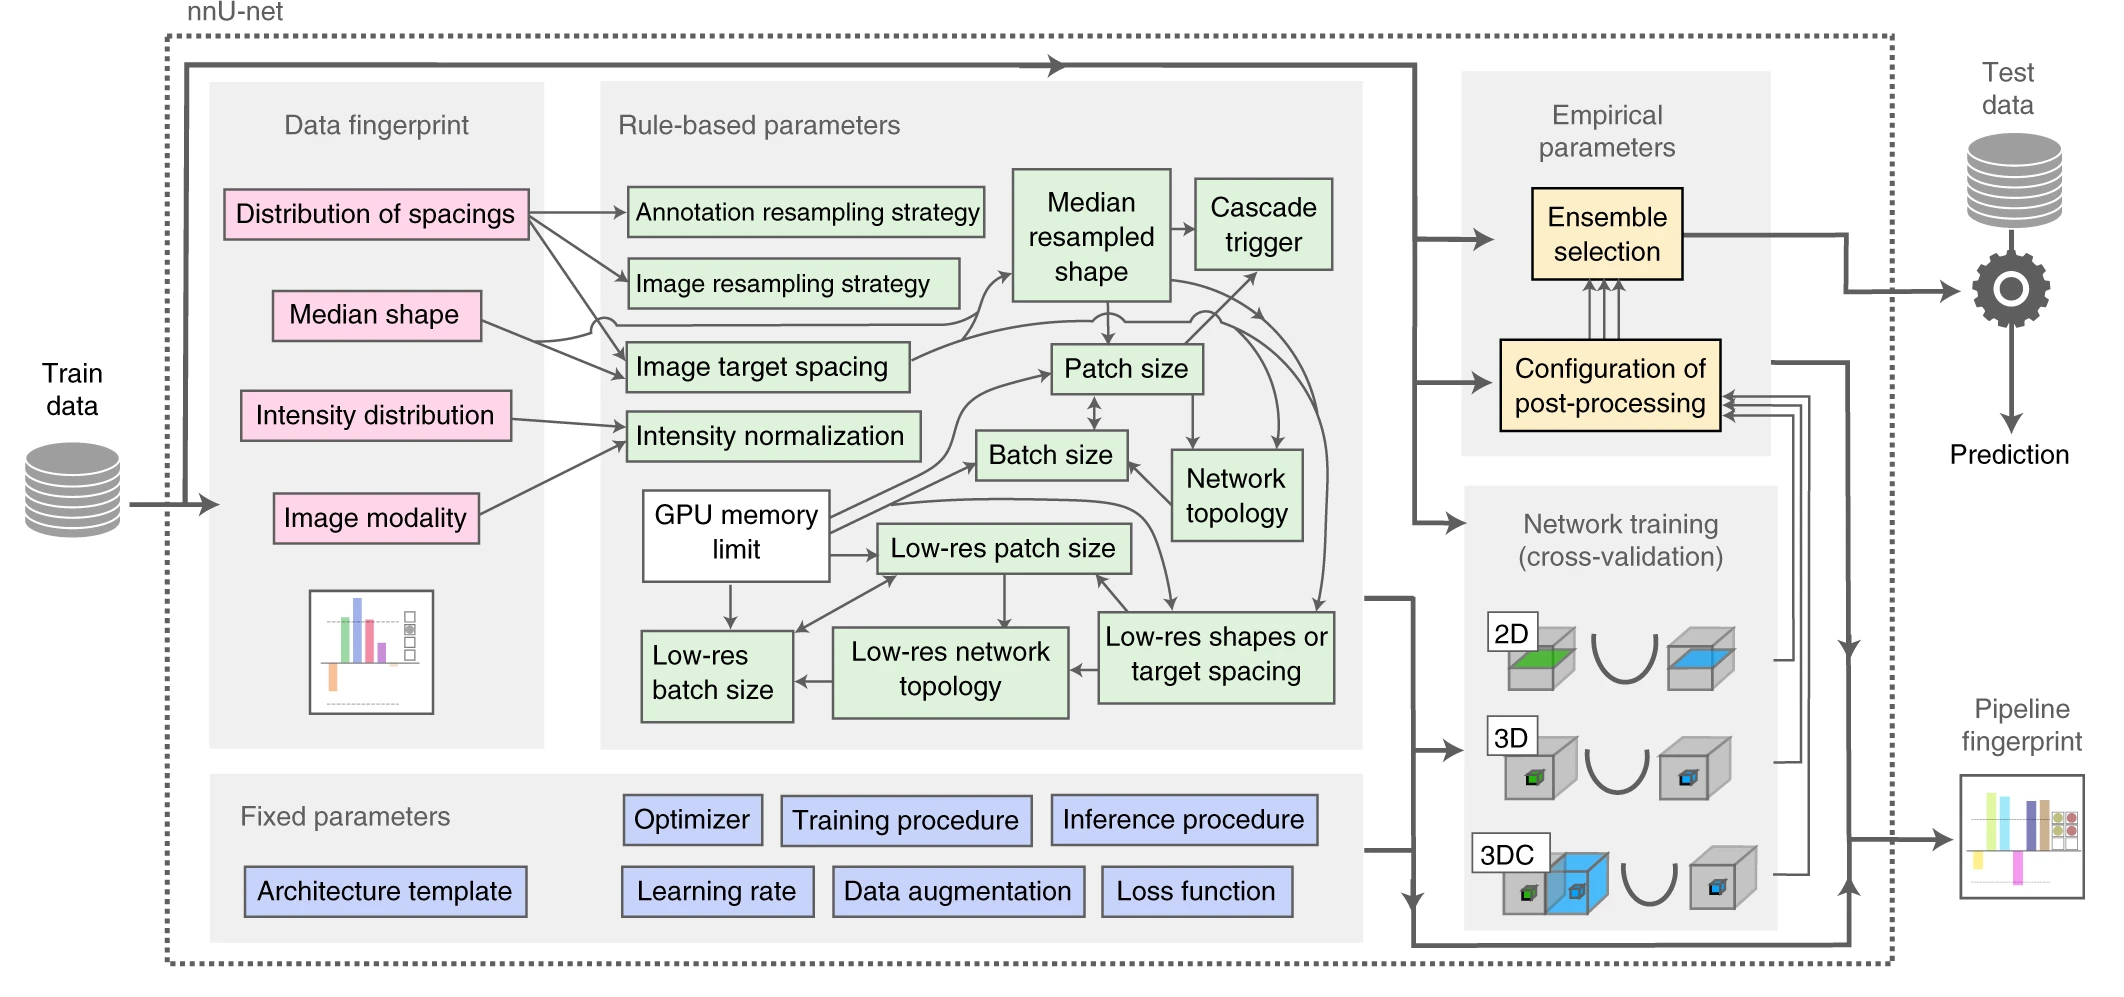
\includegraphics[width=\linewidth]{images/nnunet-arch}
 \caption{A diagram of the nnU-Net procedure of creating a training configuration. \cite{isenseeNnUNetSelfconfiguringMethod2021}}
 \label{fig:nnunet-arch}
 \end{figure}
 
 nnU-Net has demonstrated exceptional performance, establishing itself as a state-of-the-art solution in a variety of CT and MRI segmentation tasks. nnU-Net is a hugely important tool for both academia and industry, as it allows for creating well-tuned baseline models with very little manual intervention or technical expertise.
 
 Furthermore, nnU-Net exemplifies the critical role of preprocessing and parameter tuning in improving model performance, particularly when working with small datasets. This is the cornerstone of this thesis: improving data efficiency through preprocessing. The success of nnU-Net serves as a validation of this approach.
 
 \subsubsection{U-Net++}
 
In standard U-Net, skip connections link encoder layer outputs to decoder layer inputs through basic concatenation operations. This approach leaves room for more intricate integration of the decoder and encoder outputs. Additionally, U-Net only merges features at corresponding levels of the encoder and decoder. An enhancement to this could be to allow each decoder layer access to features from multiple encoder layers. U-Net++ \cite{zhou2019unetplusplus} takes advantage of these opportunities with a flexible architectural design.

In U-Net++, skip connections are reimagined as a network of convolutional layers. This setup connects each encoder layer to its respective decoder layer through multiple convolutional layers.  This enhances the information fed into the skip convolutional layers. Additionally, the outputs of these skip connections are further upscaled and fed into the subsequent decoder layers. This design results in a significantly more complex network architecture. Here, each decoder layer not only receives features from its direct encoder counterpart but also from all deeper encoder layers. This multifaceted connection system is visually represented in \figref{fig:unetpp-arch}.
 
 In U-Net++, skip connections are reimagined as a network of convolutional layers instead of simple concatenation. Moreover, outputs from each encoder layer (except the first) are upscaled and then supplied as additional inputs to the skip connections of the preceding layer. The outputs of the skip connections themselves are also upscaled and given to the next corresponding decoder layer. Thus, each decoder layer not only receives features from its direct encoder counterpart but also from all deeper encoder layers. This architecture is presented in \figref{fig:unetpp-arch}.
 
 \begin{figure}[t!]
 \centering
 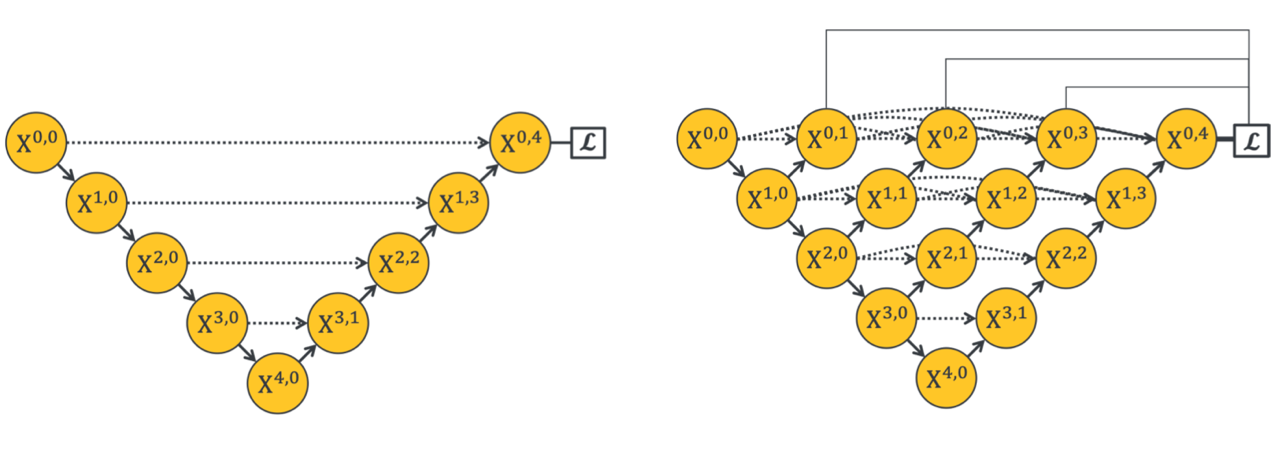
\includegraphics[width=\linewidth]{images/unetpp-arch}
 \caption{A comparison between U-Net (left) and U-Net++ (right). Each node in the graph represents a convolutional layer. The dashed arrows represent skip connections, while full arrows are downsampling or upsampling operations. \cite{zhou2019unetplusplus}}
 \label{fig:unetpp-arch}
 \end{figure}
  
There are several advantages to U-Net++ over U-Net. Each decoder layer has access to multi-scale features of the input image and thus can produce more accurate outputs. Conceptually, U-Net++ can be viewed as an ensemble of U-Nets with varying depths, which helps in faster convergence compared to a standard U-Net of similar depth. Further, instead of finding the optimal U-Net depth, due to the flexibility of neural networks, U-Net++ learns the optimal depth during training. This makes U-Net++ more flexible, requiring fewer design decisions. However, U-Net++ has a higher parameter count and does not necessarily enhance data efficiency. In some cases, its performance benefits can be matched or surpassed by a well-preprocessed and tuned U-Net \cite{isenseeNnUNetSelfconfiguringMethod2021}.

\subsection{Mask R-CNN}

Earlier in the chapter we mentioned that CNN-based segmentation networks generally consist of encoder and decoder stages. Segmentation architectures such as U-Net employ a decoder that progressively upsamples the feature maps to construct a segmentation map. This differs from how object detection decoders work.

Object detection aims to find the location of an object in an image. Instead of classifying each pixel as in segmentation, object detection typically outputs the coordinates of a bounding box surrounding the object. In technical terms, the output is not an image but rather a vector of four numbers for each object. As such, the decoders in object detection networks are usually much shallower and employ fully connected layers instead of convolutional layers.

Despite these differences, both object detection and segmentation networks share similar encoder designs. Mask R-CNN \cite{heMaskRCNN2017b} takes advantage of this to combine object detection and segmentation into a single network. In Mask R-CNN, a standard CNN encoder generates a feature map from an input image. This map is then given to two parallel decoders: one for segmentation and the other for object detection. The segmentation decoder, akin to those in standard segmentation networks, uses convolutional layers and upsampling to generate a segmentation map for each object. The detection decoder, in contrast, employs downsampling and fully connected layers to output the bounding box and class label of each object. The Mask R-CNN architecture can be seen in \figref{fig:maskrcnn-arch}.

 \begin{figure}[t!]
 \centering
 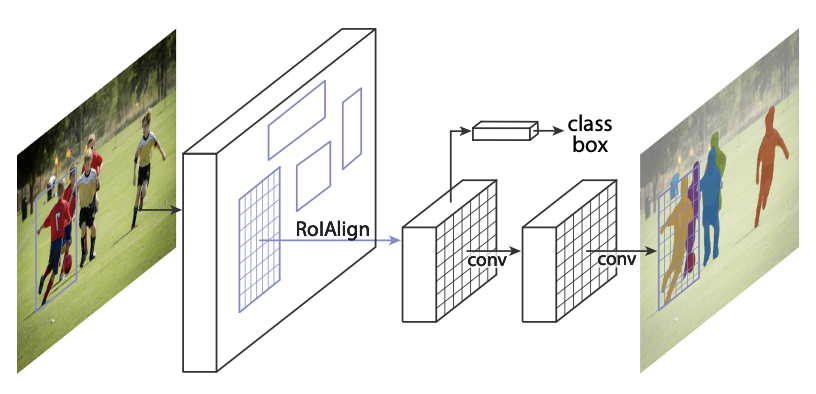
\includegraphics[width=0.6\linewidth]{images/maskrcnn-arch}
 \caption{A diagram of the Mask R-CNN architecture. Two parallel decoder branches are used to achieve segmentation and object detection simultaneously. \cite{heMaskRCNN2017b}}
 \label{fig:maskrcnn-arch}
 \end{figure}

Consequently, for every detected object, Mask R-CNN provides a bounding box, a class label, and a segmentation mask. The network is trained using a composite loss function, optimizing for segmentation, detection, and classification simultaneously.

The integration of these tasks in Mask R-CNN takes advantage of synergies between them. The information learned for classifying an object is relevant to its detection. Similarly, by using a bounding box the segmentation decoder can focus on the relevant portion of the image and be invariant to the scale of the object on the image. This joint learning approach enhances performance across all tasks compared to training separate networks for each task. However, Mask R-CNN's complexity can pose challenges, particularly when trained on very small datasets, where simpler segmentation-focused architectures like U-Net might be more effective.

\subsection{Other Notable Segmentation CNNs}

A central challenge in CNN-based segmentation is balancing spatial information with feature complexity. As the network increases the feature map depth and decreases width and height, spatial information is erased but more complex features can be detected on the image. Effective segmentation requires both elements. While U-Net addresses this with skip connections, other architectures use different methods to integrate multi-scale features.

One approach involves pyramid pooling, as utilized in PSPNet \cite{zhao2017pspnet}. Initially, PSPNet uses a standard encode to create a feature map. This map is then rescaled to various sizes, and each rescaled map undergoes processing through a series of convolutional layers. The resulting outputs from these layers are resized to a uniform spatial dimension and concatenated. This combined feature map is then fed into a decoder to produce the final segmentation map.

Pyramid pooling is also employed by DeepLabV3 \cite{chen2017rethinking} albeit in a different way. Like in PSPNet, the encoder first creates a feature map. This feature map then goes through a series of parallel layers that each use an atrous convolution. In atrous convolution, the kernel is dilated by introducing gaps between its values. During each sliding window step, the gaps are ignored and the result is convolved regularly for non-empty kernel values. This technique enables covering a larger area of the image without increasing kernel parameters. Each parallel layer uses different gap sizes in the kernel, creating multi-scale features. These features are upscaled, merged, and further decoded into a segmentation map.

MA-Net \cite{manet} takes a different route by incorporating an attention mechanism for combining multi-scale features. Rather than directly concatenating in skip connections like U-Net, MA-Net introduces a multi-scale attention block. This block aims to capture the interdependencies of different features to focus on more salient ones before they are concatenated to the decoder layer input. Additionally, the final decoder layer is processed through a position-wise attention block to highlight significant features in specific image locations. MA-Net has shown performance improvements in liver tumor segmentation on CT images compared to U-Net and U-Net++.

\section{Fully Connected Transformers for Medical Image Segmentation}

So far most of this chapter dealt with CNNs. However, another class of networks --- transformers \cite{attnAllYouNeed} --- has recently gained traction and even surpassed the segmentation quality of CNNs for many tasks. The key to the transformer's impressive performance is the ability to support very deep neural networks. Empirical observations suggest that with enough data, network performance tends to increase with the depth of the network. Hence, transformers have become state-of-the-art in tasks where a large amount of data is available. Notably, current transformers used in natural language processing contain more than 100 layers and trillions of parameters, orders of magnitude more than CNN-based models.

Transformers first became broadly used in the field of natural language processing and achieved groundbreaking results in text generation, machine translation, and understanding natural language. Broadly, transformers employ a combination of regular (non-convolutional) fully connected layers and attention mechanisms, which are the key to their success. Attention allows a layer to learn the interdependencies between parts of its input or across different input values. In linguistic contexts, this leads to a more nuanced understanding of syntactic relationships, enabling the network to learn concepts such as the interplay between subjects and objects or the likelihood of certain adjectives preceding specific nouns.

\subsection{Attention}

For each element $x_i$ of an input sequence of length $n$, an attention mechanism aims to produce a vector $v_i = (v_{i1}, v_{i2}, \cdots, v_{in})$ where $v_{ij}$ measures how dependent $x_i$ is on $x_j$. In a natural language scenario, if we consider a sentence as our input sequence, this mechanism can be envisioned as going word by word, and for each word producing relevance scores for every other word in the sentence. For instance, in the sentence ``Susan has a brown dog that she loves.'', the word ``she'' should have a high relevance score for ``Susan'', and a low score for ``brown'' since it is not pertinent to encoding the meaning of ``she'' in this sentence.

Mathematically, attention can be expressed as a series of matrix multiplications. First, each input sequence element is transformed into a query vector. This transformation represents a learned encoding by the network, converting an input element into a lower-dimension vector. The query serves to identify the current input element in the sequence. Let $X$ be an input matrix where each row is a new element of the sequence. Let $W_Q$ be a matrix of weights learned by the network that encodes each element of the input sequences into a vector. The query matrix $Q$ can then be calculated as
\begin{equation}
Q = W_Q X,
\end{equation}
where each row $Q_i$ represents the query for $X_i$. Remember that the goal of attention is to score the relevance between an input element $X_i$ and some other element $X_j$ of the same input sequence. Having encoded each element $X_i$ in the form of $Q_i$, we need to similarly encode each $X_j$ in a different matrix $K$ where $K_j$ is called the \textbf{key} for some input sequence element $X_j$. We can do so as
\begin{equation}
K = W_K X,
\end{equation}
where $W_K$ is another weight matrix that the model optimizes during training. Given $K$ and $Q$, we can compute the relevance scores for every combination of input elements $x_i$ and $x_j$ as
\begin{equation}
A = Q K^T.
\end{equation}
Here, $A_{ij}$ represents the relevance score between $x_j$ and $x_i$. It is important to note that this is only one of many ways the matrix $A$ can be calculated. In practice, $A$ is scaled to be in $[0, 1]$ or transformed in some other way.

Finally, to get the output $Z$ of the self-attention layer, we weigh each element of the original input sequence $X$ by the attention scores $A$:
\begin{equation}
Z = A V,
\end{equation}
$Z$ consists of $X$ elements weighted by how relevant they are to the encoding of the whole sequence. Visually, this process for one element of the input sequence can be seen in \figref{fig:attention-explainer}.

 \begin{figure}[t!]
 \centering
 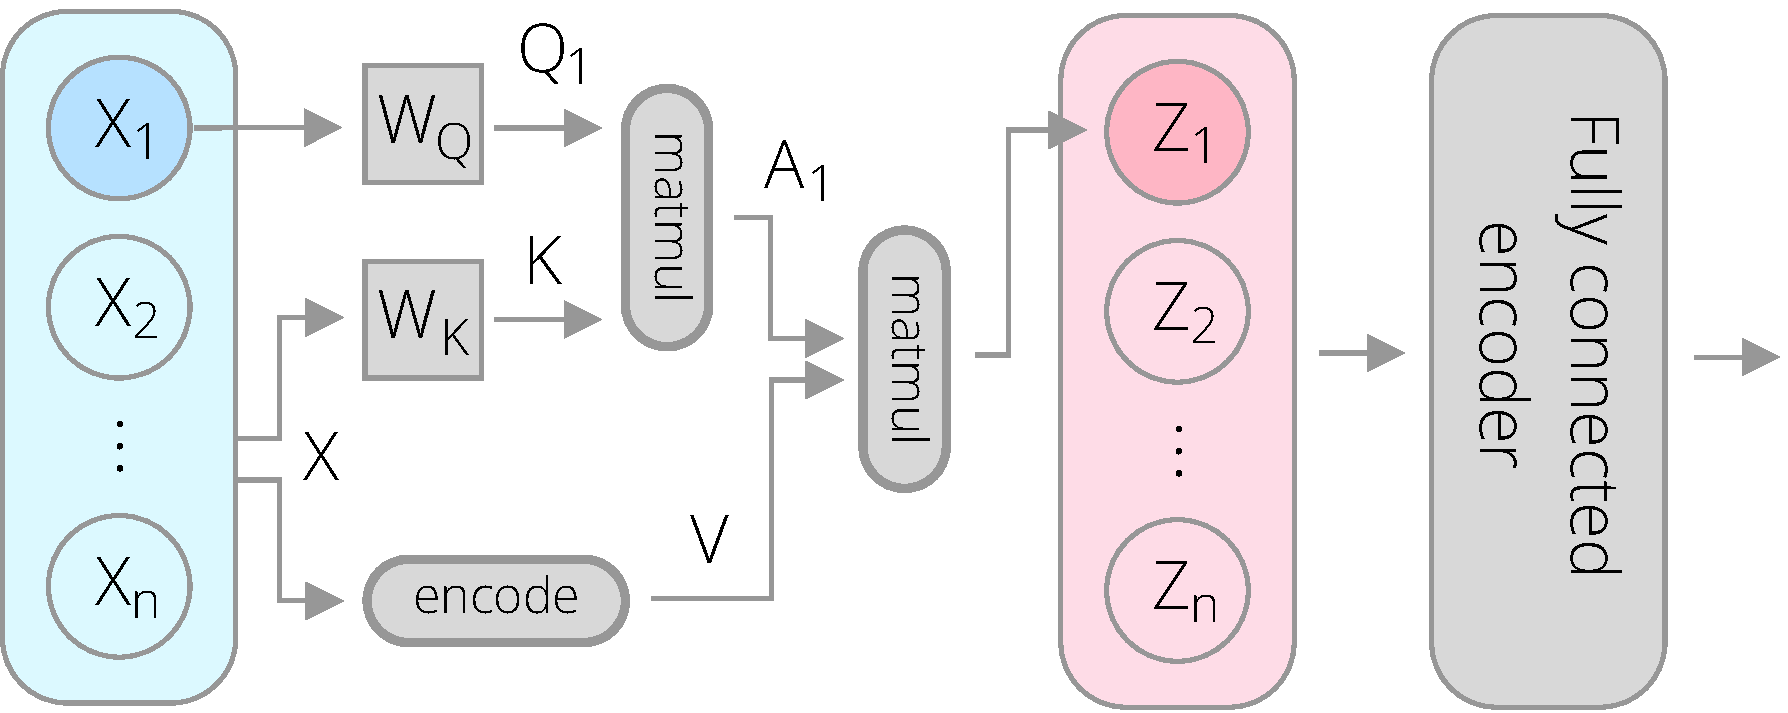
\includegraphics[width=0.8\linewidth]{images/attention-explainer}
 \caption{A visualization of a single encoder layer in a transformer network. This shows the encoding process for one element of the input sequence.}
 \label{fig:attention-explainer}
 \end{figure}
 
 Encoder and decoder layers in a transformer include an attention layer followed by a fully connected layer. In the encoder, the attention layers are generally \textit{self-attention}, where both the key and the query come from the input sequence. In contrast, the decoder layers employ both self-attention and \textbf{encoder-decoder attention}. In the latter, the keys and values come from the encoded features of the last layer of the encoder. Finally, each attention layer performs $Z$ calculation multiple times using different $W$ and $K$ weights, and the weighted values are concatenated together. This design enables the network to simultaneously learn and apply various types of attention within each individual layer.
 
 \subsection{Positional Encoding}
 
The position of each word in a sentence carries important information. The sentence ``The yellow notebook is on top of the red notebook.'' has a different meaning than ``The red notebook is on top of the yellow notebook.'', even though both sentences contain the same words. To capture this in transformers, the position of each input element is encoded and included as part of the input.
 
Each input sequence element index is mapped to a matrix via a function $f : \mathbb{Z}^{+} \rightarrow \mathbb{R}^d$ where $d$ is the dimensionality of the layer's input. Mapped that way, the positional encoding can simply be concatenated to the layer's input with no additional changes in the network. While it is possible for this encoding function to be represented as neural network layers and learned during training, a common approach is to use a predefined, fixed function. For instance, in cite{attnAllYouNeed}, given an element index $pos$, the $i$-th element of the positional encoding is calculated as
\begin{equation}
PE(pos, i) = \begin{cases}
	\sin(pos/1000^{2i/d}), & \text{$i$ is even}\\
	\cos(pos/1000^{2i/d}), & \text{$i$ is odd}\\
\end{cases}.
\end{equation}
The choice of positional encoding functions is guided by their numerical characteristics, ensuring they are efficiently processed by the neural network.
  
 \subsection{Adapting Transformers to Image Segmentation}
 
 Convolutional Neural Networks (CNNs) have traditionally dominated image processing due to their efficiency in handling large inputs. Consider a $128 \times 128$ pixel image which, when flattened into a row vector, results in 16,384 elements. In a fully connected network, where each input element connects to every output element, this translates into $16,384^2$ parameters for just one layer. Even if the image were to be heavily downscaled and ignore the loss of information this would create, managing such a network on current GPUs is infeasible.
 
 Transformers that use fully connected layers face a challenge when applied to image data due to this very issue. The key solution, as utilized in the Vision Transformer (ViT) \cite{dosovitskiy2021an}, is treating an image as a sequence of small patches, allowing the image to be processed similarly to text.
 
 ViT, primarily designed for image classification, begins by partitioning each image into uniform square patches (e.g. $32 \times 32$ pixels). The patches, ordered starting from the top-left of the image, form an input sequence $X$. Each patch is then flattened to a row vector and given to a fully connected layer to encode it as a $d$-dimensional vector. Then, a $d$-dimensional positional encoding is added to the encoding as a function of the patch index. The resultant matrix serves as the input for the encoder, which operates identically to a standard transformer network. This architecture can be seen visually in \figref{fig:vit-arch}.
 
  \begin{figure}[t!]
 \centering
 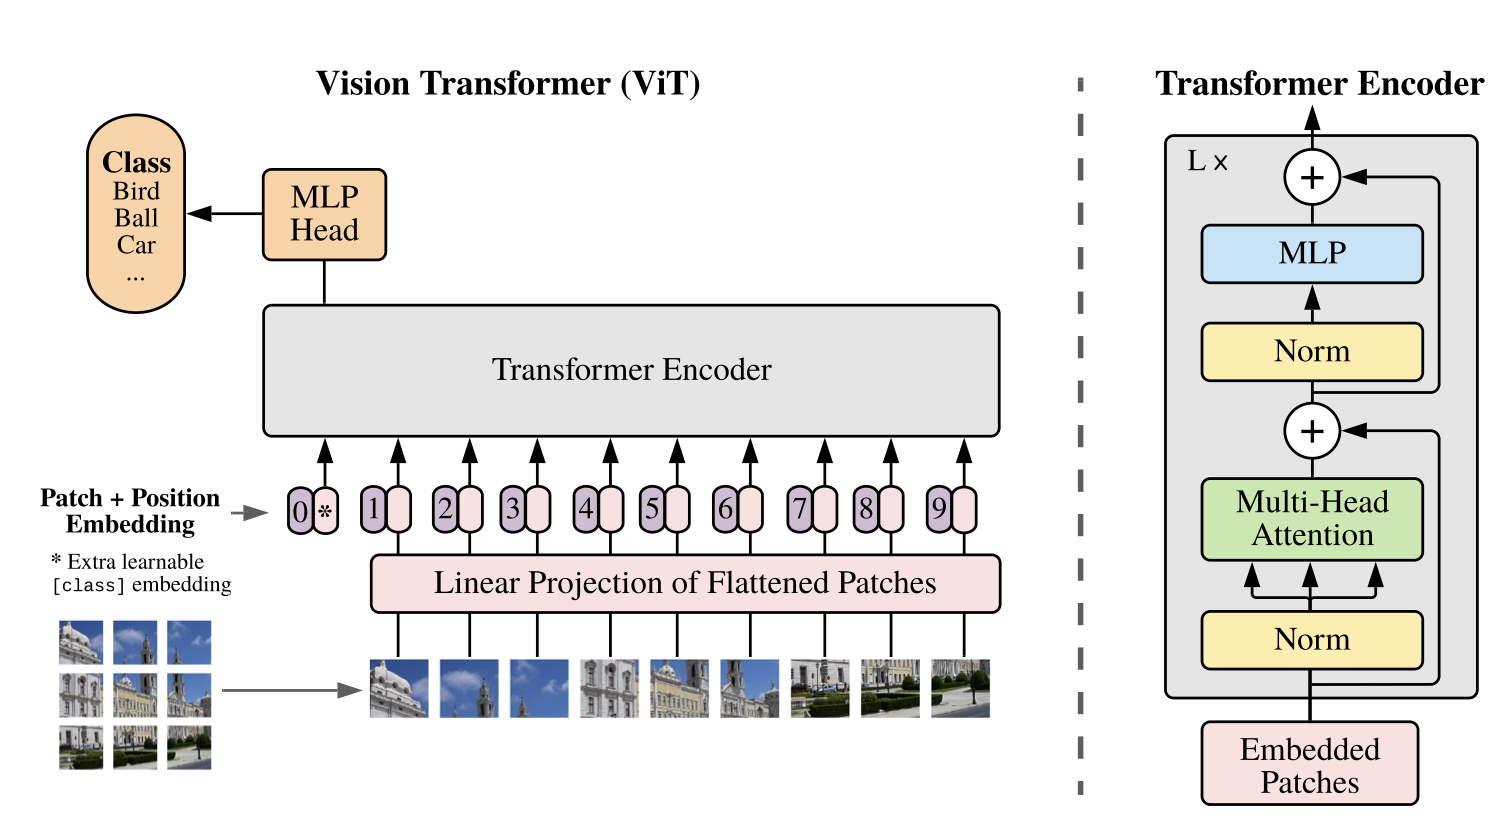
\includegraphics[width=\linewidth]{images/vit-arch}
 \caption{The ViT architecture for image classification. \cite{dosovitskiy2021an}}
 \label{fig:vit-arch}
 \end{figure}
 
 While ViT originally used a classification decoder, it is possible to combine the ViT encoder with a segmentation decoder to obtain a segmentation map. There are several ways this has been achieved. For instance, the Segmentation Transformer (SETR) \cite{SETR} introduces two distinct CNN-based segmentation decoders connected to a ViT encoder. The first variant follows a conventional convolutional decoder design, where the encoder's output goes through a series of upsampling and convolutional layers, producing a segmentation map in the original image resolution. The second decoder variant is similar to the way FCN works --- outputs from various encoder layers are resized to a uniform resolution, merged, and then decoded into a segmentation map.

 Later transformer-based segmentation networks modified the ViT encoder as well. For instance, the authors of the Swin Transformer \cite{liu2021Swin} argue that neural networks for computer vision need to be built with translation and scale invariance in mind. Swin Transformer starts with small patches, similar to ViT, but in each successive encoder layer neighboring patches are merged. Rather than computing self-attention within individual patches, Swin uses non-overlapping windows of multiple patches to perform self-attention. This ensures that Swin’s computational demand increases linearly with image size, a significant improvement over ViT’s exponential growth. A key aspect of Swin is that each successive layer shifts the window by half of the window size. This allows self-attention between two different windows and more global information about the image. Finally, Swin's encoder output is fed into a DeepLab-like decoder to produce the segmentation map.
 
 Transformers have demonstrated exceptional performance in image segmentation, particularly in large datasets and benchmarks with upwards of 20,000 natural images \cite{liu2021Swin, SETR, chen2022vitadapter}. However, their advantage is less pronounced in smaller datasets. This aligns with observations from \cite{attnAllYouNeed} --- convolutional layers have properties that are naturally a good fit for extracting information out of images. Transformers need to compensate for their lack of convolutions by using more layers. However, as we will see in the next chapter, there is a relationship between the number of parameters of a network and the number of samples required to train that network.

